\documentclass[11pt,oneside]{book}
\usepackage{fontspec}
\usepackage{xeCJK}
\setmainfont{Latin Modern Roman}
\setCJKmainfont[ItalicFont={Noto Serif CJK TC},BoldItalicFont={Noto Serif CJK TC Bold}]{Noto Serif CJK TC}
\setCJKsansfont{Noto Sans CJK TC}
\setCJKmonofont{Noto Sans Mono CJK TC}
\newfontfamily\proseunicodefont{DejaVu Serif}
\usepackage[margin=1in]{geometry}
\usepackage{microtype}
\usepackage{amsmath,amssymb,amsthm,mathtools,bm}
\usepackage{graphicx}
\usepackage{xcolor}
\usepackage{booktabs}
\usepackage{array}
\usepackage{longtable}
\usepackage{enumitem}
\usepackage{float}
\usepackage{caption}
\usepackage{hyperref}
\usepackage{fancyhdr}
\usepackage{tikz}
\usetikzlibrary{arrows.meta,positioning,calc,decorations.pathmorphing}

\hypersetup{
  colorlinks=true,
  linkcolor=blue!50!black,
  urlcolor=blue!50!black,
  citecolor=blue!50!black
}

\setlength{\parskip}{0.5em}
\setlength{\parindent}{0pt}
\setlist[itemize]{topsep=0.25em,itemsep=0.2em}
\setlist[enumerate]{topsep=0.25em,itemsep=0.2em}
\setlength{\headheight}{40pt}
\numberwithin{equation}{chapter}

\newtheorem{theorem}{定理}[chapter]
\newtheorem{proposition}[theorem]{命題}
\newtheorem{lemma}[theorem]{引理}
\newtheorem{corollary}[theorem]{推論}
\theoremstyle{definition}
\newtheorem{definition}[theorem]{定義}
\newtheorem{example}[theorem]{例}
\theoremstyle{remark}
\newtheorem{remark}[theorem]{註}

\providecommand{\ket}[1]{\left\lvert#1\right\rangle}
\providecommand{\bra}[1]{\left\langle#1\right\rvert}
\providecommand{\braket}[2]{\left\langle#1\,\middle|\,#2\right\rangle}
\providecommand{\expect}[1]{\left\langle#1\right\rangle}
\newcommand{\lectureoverview}[1]{\paragraph{概述。} #1}

\makeatletter
\newcommand{\course@headerfont}{\normalfont\small\itshape}
\newcommand{\course@pagefont}{\normalfont\small}
\newcommand{\course@headerraise}{14pt}
\newlength{\course@headerboxheight}
\setlength{\course@headerboxheight}{\dimexpr\headheight-\course@headerraise-9pt\relax}
\newcommand{\course@leftheadbox}[1]{%
  \raisebox{\course@headerraise}{%
    \parbox[t][\course@headerboxheight][t]{0.82\textwidth}{%
      \raggedright\course@headerfont\strut\MakeUppercase{#1}\strut%
    }%
  }%
}
\newcommand{\course@rightheadbox}[1]{%
  \raisebox{\course@headerraise}{%
    \parbox[t][\course@headerboxheight][t]{0.82\textwidth}{%
      \raggedleft\course@headerfont\strut\MakeUppercase{#1}\strut%
    }%
  }%
}
\renewcommand{\chaptermark}[1]{\markboth{\MakeUppercase{\chaptername\ \thechapter.\ #1}}{}}
\renewcommand{\sectionmark}[1]{\markright{\MakeUppercase{\thesection\hspace{0.4em}#1}}}
\fancyhf{}
\fancyhead[L]{\course@leftheadbox{\leftmark}}
\fancyhead[R]{\course@pagefont\thepage}
\renewcommand{\headrulewidth}{0.5pt}
\pagestyle{fancy}
\fancypagestyle{plain}{%
  \fancyhf{}
  \fancyhead[L]{\course@leftheadbox{\leftmark}}
  \fancyhead[R]{\course@pagefont\thepage}
  \renewcommand{\headrulewidth}{0.5pt}
}
\makeatother

% Video2Book editorial provenance macros
\newenvironment{classroomqa}{%
  \par\medskip\noindent\begin{minipage}{\linewidth}\small\hrule\medskip
}{%
  \medskip\hrule\end{minipage}\par\medskip
}
\newcommand{\audiencequestion}[1]{\noindent\textbf{聽眾提問。} #1\par\smallskip}
\newcommand{\lecturerresponse}[1]{\noindent\textbf{回答。} #1\par}
\newcommand{\lecturetimestamp}[1]{\footnote{講課時間： #1.}}
\newcommand{\lectureframe}[1]{\par\smallskip{\centering\footnotesize\itshape 講課畫面： #1.\par}}
\newcommand{\editorialnote}[1]{\footnote{編者說明： #1}}

\renewcommand{\contentsname}{目錄}
\renewcommand{\chaptername}{章}
\renewcommand{\figurename}{圖}
\renewcommand{\tablename}{表}
\renewcommand{\proofname}{證明}
\renewcommand{\bibname}{參考文獻}
\emergencystretch=2em
\pdfstringdefDisableCommands{\def\proseunicodefont{}}

\geometry{paperwidth=177.6mm,paperheight=252mm,left=16mm,right=16mm,
 top=18mm,bottom=18mm,includeheadfoot,headheight=28pt,headsep=7mm,footskip=9mm}
\usepackage{scrextend}
\changefontsizes[17pt]{12pt}
\raggedbottom
\renewenvironment{classroomqa}{\par\medskip\begingroup}{\par\endgroup\medskip}
\fancyhf{}
\setlength{\headwidth}{\textwidth}
\fancyhead[L]{\parbox{\textwidth}{\raggedright\fontsize{9}{11}\selectfont\nouppercase{\leftmark}}}
\fancyfoot[C]{\small\thepage}
\renewcommand{\headrulewidth}{0.3pt}
\fancypagestyle{plain}{\fancyhf{}\fancyfoot[C]{\small\thepage}\renewcommand{\headrulewidth}{0pt}}

\graphicspath{{../../../generated_course_notes/core/cosmology/2009_winter_legacy_cosmology/figures/}{../../../generated_course_notes/core/cosmology/2009_winter_legacy_cosmology/assets/}}
\begin{document}
\frontmatter
\hypersetup{pageanchor=false}
\begin{titlepage}
\hyphenpenalty=10000\exhyphenpenalty=10000
\thispagestyle{empty}
\begin{tikzpicture}[remember picture,overlay]
  \node[anchor=center,inner sep=0] at (current page.center) {%
    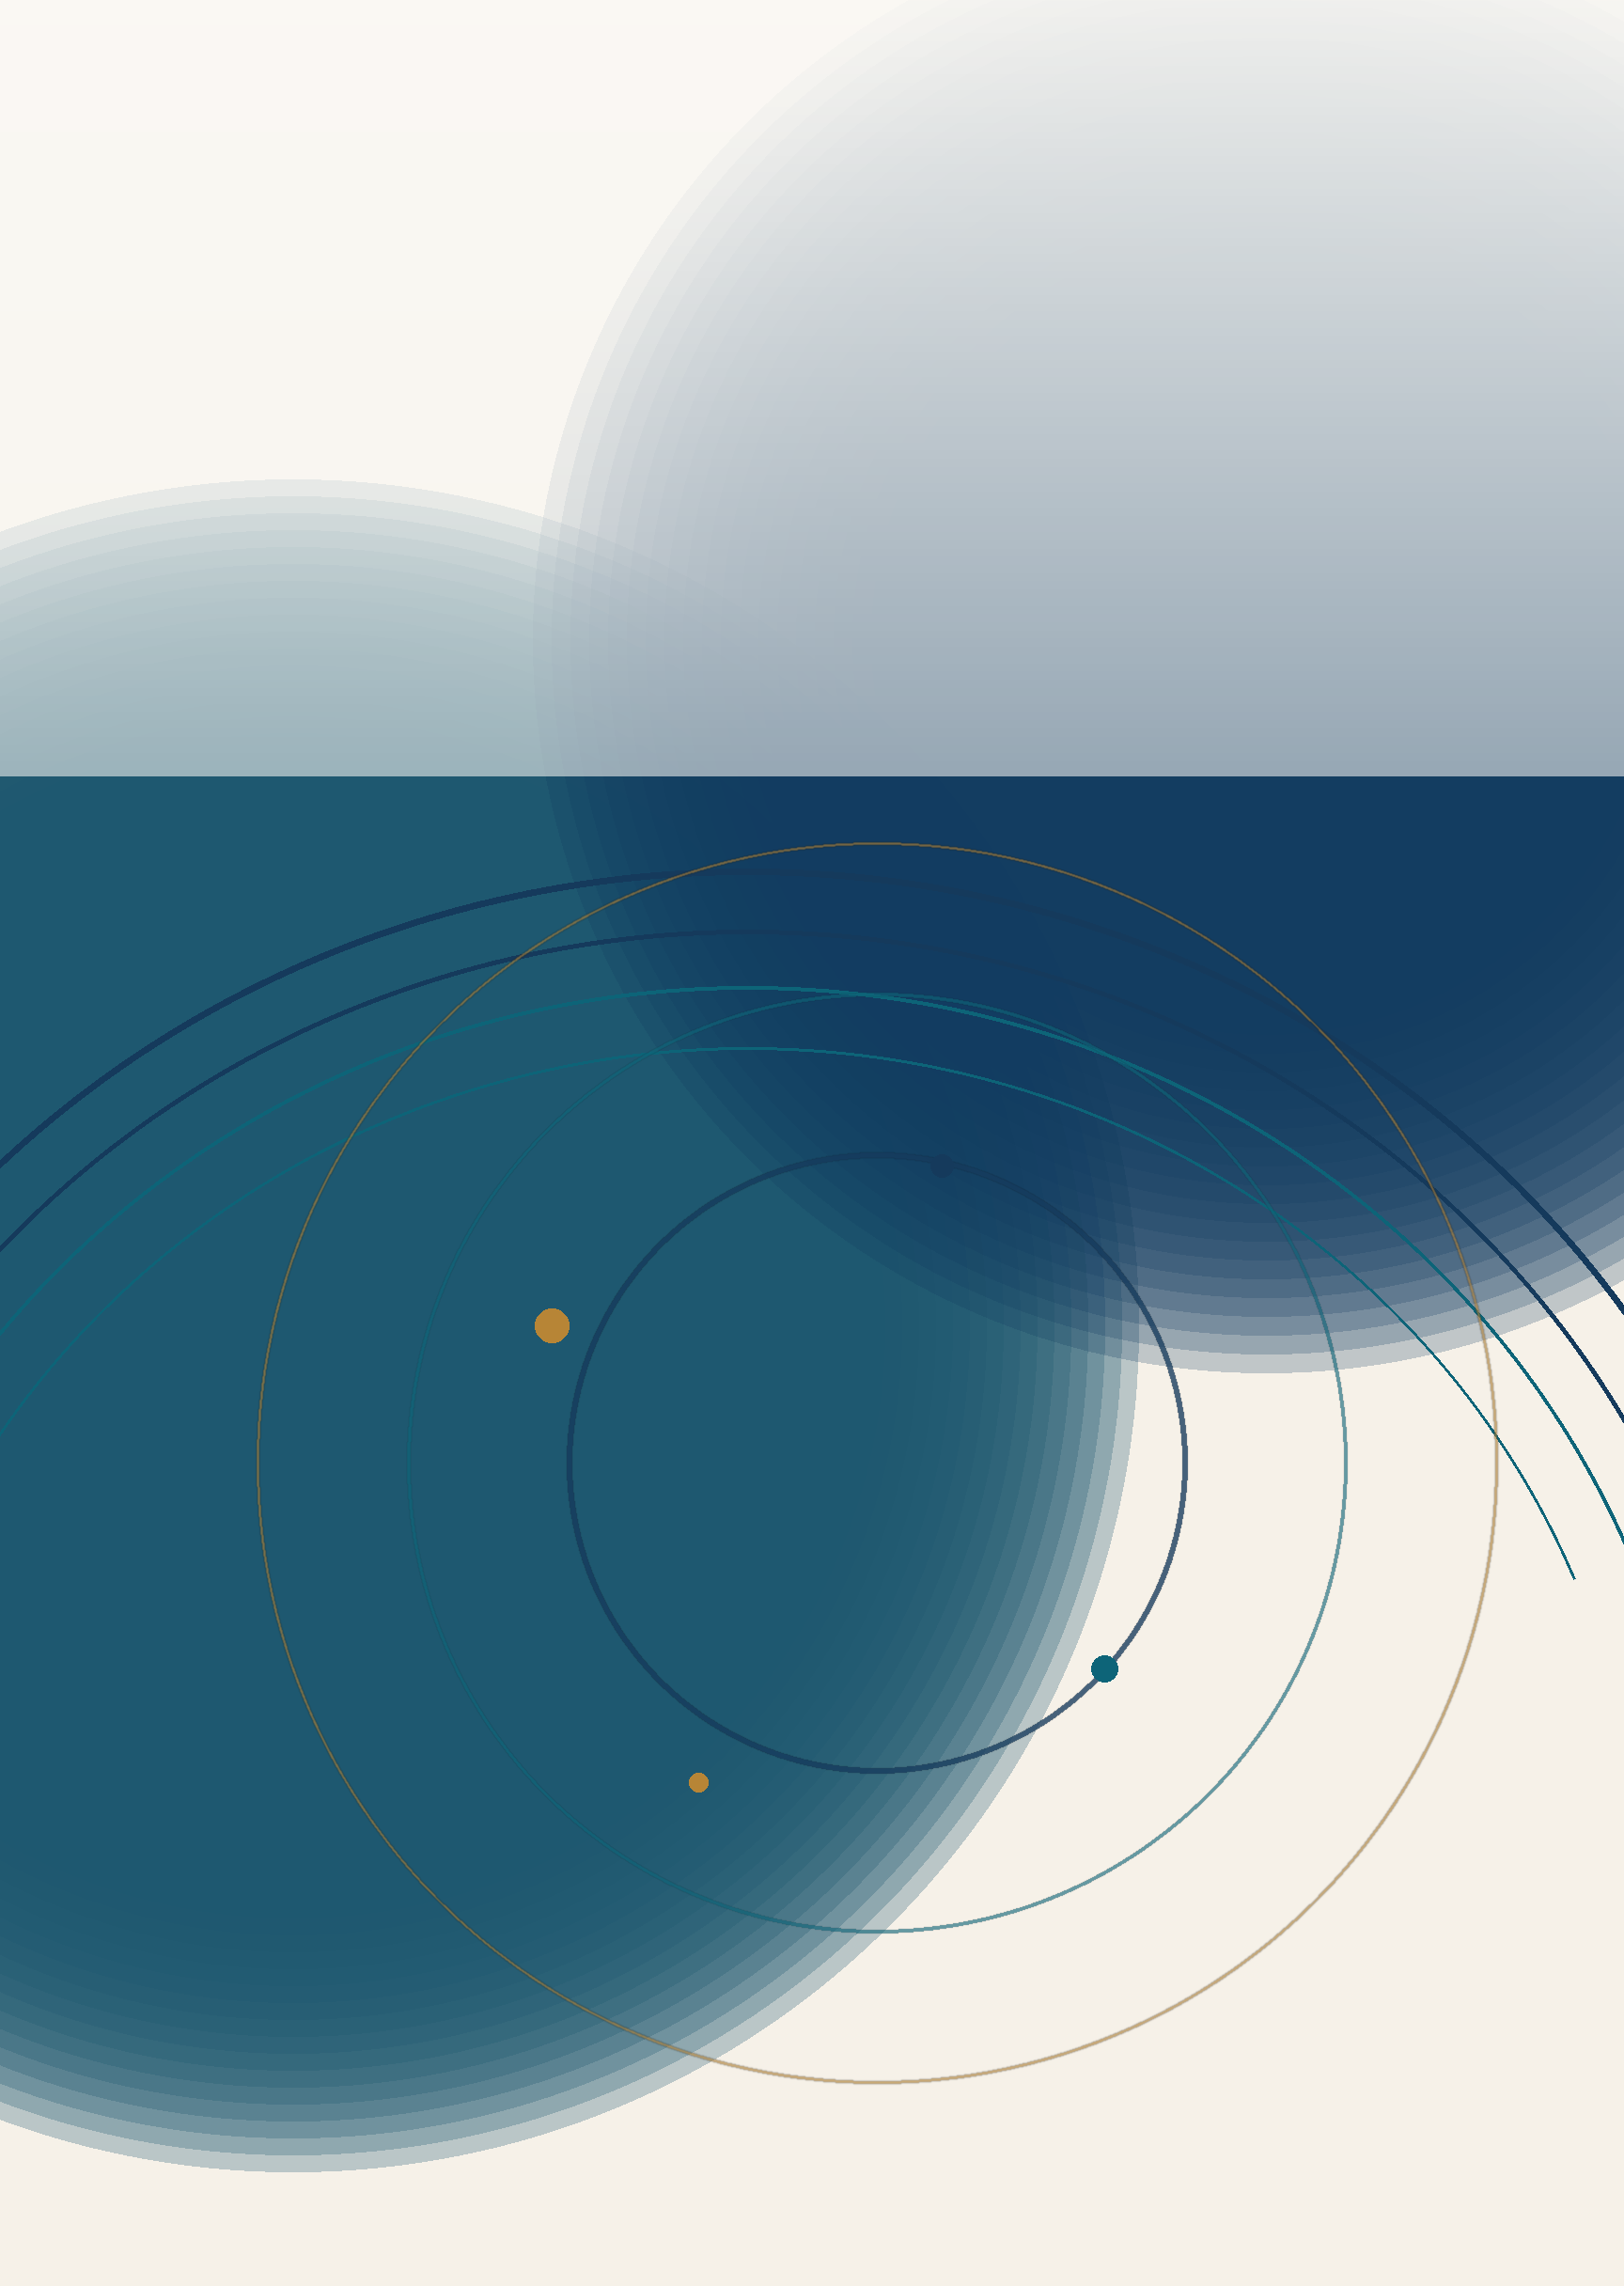
\includegraphics[height=\paperheight,keepaspectratio]{../../../generated_course_notes/core/cosmology/2009_winter_legacy_cosmology/assets/cover-art.png}%
  };
  \node[
    anchor=north west,
    align=left,
    text width=0.78\paperwidth,
    fill=white,
    fill opacity=0.9,
    rounded corners=8pt,
    inner xsep=10pt,
    inner ysep=8pt
  ] at ([xshift=0.08\paperwidth,yshift=-0.06\paperheight]current page.north west) {%
    {\fontsize{30}{33}\selectfont\bfseries\color{black!88} 宇宙學\\[0.85em]}
    {\large\color{black!72} 繁體中文版 / 2009年冬季・舊版宇宙學}
  };
  \node[
    anchor=south west,
    align=left,
    text width=0.68\paperwidth,
    fill=white,
    fill opacity=0.82,
    text opacity=1,
    rounded corners=6pt,
    inner sep=12pt
  ] at ([xshift=0.08\paperwidth,yshift=0.08\paperheight]current page.south west) {%
    {\normalsize\color{black!78} 原講授：Leonard Susskind\\[0.35em]}
    {\small\color{black!72} 講義輔助版本：\href{https://lazying.art}{LazyingArt LLC} / \href{https://github.com/lachlanchen/Video2Book}{Video2Book}}
  };
\end{tikzpicture}
\mbox{}
\end{titlepage}
\hypersetup{pageanchor=true}

\clearpage
\chapter*{關於本講義}
這些經獨立編輯的配套講義依據 Leonard Susskind 的講課內容編寫。內容根據機器轉錄稿、字幕及選取的黑板畫面重建，並與可取得的原始資料核對。這些講義並非 Susskind 教授的原稿，也未經他審閱或認可。

本版本由 \href{https://lazying.art}{LazyingArt LLC} 使用開源的 \href{https://github.com/lachlanchen/Video2Book}{Video2Book} 工作流程編製。機器轉錄稿另行提供，其中可能有辨識錯誤。編輯上的釐清與實質性的重建均以腳註標示。
\clearpage
\tableofcontents
\mainmatter
\chapter{膨脹宇宙的幾何}

重點在於膨脹宇宙及其幾何。我們要先說明空間膨脹的意義，再探討是什麼驅動了膨脹。牛頓力學\(F=ma\)宇宙學會在稍後討論；接著才會把幾何與動力學結合，建立完整的 Friedmann--Robertson--Walker 架構。

\section{膨脹直線上的共動座標}

先從最簡單的例子開始：一維空間，而不是時空。想像一條無限長的直線，上面有等間距排列的星系。座標 \(x\) 此時還不表示物理距離，只用來標記星系。可以把 \(x\) 想成某個星系的名稱；即使整個排列伸展或收縮，這個名稱仍附著在該星系上。

設從標記為 \(x=0\) 的星系到標記為 \(x=1\) 的星系，其物理距離為 \(a\)。那麼，任意兩個星系之間的物理距離為
\begin{equation}
d=a\,\Delta x.
\end{equation}
座標差 \(\Delta x\) 只是標籤之間的差值。因子 \(a\) 會把這個標籤差值轉換成以米尺量得的實際距離。

現在把這條直線想像成一根正在伸展的彈性線。標籤仍隨星系移動，但相鄰星系之間的距離會隨時間改變。同樣的關係式變成
\begin{equation}
d(t)=a(t)\,\Delta x.
\end{equation}
在這個階段，均勻性只表示相鄰星系在各處的間距都相等，儘管這個共同間距可能隨時間改變。

\section{哈勃定律與中心的不存在}

若要找出兩個固定星系的相對速度，就固定這一對星系，使 \(\Delta x\) 不隨時間改變。微分後得到
\begin{align}
\dot d &= \dot a\,\Delta x \\
       &= \frac{\dot a}{a}\,a\,\Delta x \\
       &= \frac{\dot a}{a}\,d.
\end{align}
定義
\begin{equation}
H(t)\equiv \frac{\dot a}{a},
\end{equation}
則有
\begin{equation}
\dot d = H(t)\,d.
\end{equation}
這就是哈勃定律。

歷史上使用的「``哈勃常數''」一詞容易造成誤解。這個量在空間中為常數，而不是在時間中為常數。在某一時刻，它對所有星系都相同；但一般而言，它會隨宇宙演化而改變。稱它為哈勃參數更恰當。

這條定律表示，距離越遠的星系，退行速度越快。但它並未指出任何中心。論證中沒有任何因素賦予 \(x=0\) 或其他任何點特殊地位。每位觀測者看到的規律都相同。因此，在這個模型中，膨脹宇宙並不是從某個特定位置爆發而成。

紅移立刻就會出現。若兩個星系彼此遠離時互相傳送光訊號，接收到的光會向紅端偏移。退行速度越大，紅移也越大。因此，譜線可以告訴我們退行速度。距離則較難測量，哈勃早期的估計也相當粗略。他最初繪製的圖並非完美直線，而是一組分散的資料點，且不確定度很大。即使如此，幾何上的原則仍從雜訊中顯現出來：退行速度與距離成正比。

\begin{classroomqa}
\audiencequestion{如果星系相距夠遠，哈勃定律是否表示它們的運動速度會超過光速？}\lecturetimestamp{00:20:23}
\lecturerresponse{是的，就退行速度而言，確實如此。你的說法是對的。我們一定會再談到這件事；它是最重要的事情之一。}
\end{classroomqa}

\section{高維度、各向同性與\(a(t)\)的時間依賴性}

加入更多空間維度，基本概念並不改變。在二維空間中，可以想像一個方格狀的星系網格，以 \((x,y)\) 標記；在三維空間中，則以 \((x,y,z)\) 標記。這些座標同樣是共動標籤：它們隨星系移動，而不是直接表示物理距離。

為什麼 \(x\) 方向的間距應該和 \(y\) 方向的間距相同？答案來自觀測。如果星系在某個方向上系統性地比其他方向更密集，天空看起來就會因方向而異。但在足夠大的尺度上，天空並非如此。這種方向上的一致性就是各向同性。

在二維空間中，兩個星系之間的距離為
\begin{equation}
d=a\sqrt{(\Delta x)^2+(\Delta y)^2},
\end{equation}
在三維空間中則為
\begin{equation}
d=a\sqrt{(\Delta x)^2+(\Delta y)^2+(\Delta z)^2}.
\end{equation}
對固定的一對星系，座標差保持不變，因此再次微分可得
\begin{equation}
\dot d=\frac{\dot a}{a}\,d.
\end{equation}
哈勃定律仍然不變。

均勻性是指空間各處都相同；各向同性是指各個方向都相同。兩者在小尺度上都不完全成立。透過銀河系觀測，和朝銀河盤面之外觀測，情況並不相同；在短距離尺度上，個別星系也不是均勻分布的。然而，對許多星系取平均後，大尺度宇宙在各處、各方向看起來都大致相同。

\begin{classroomqa}
\audiencequestion{如果速度與距離成正比，而距離又在增加，是否表示固定的一對星系必定在加速彼此遠離？}\lecturetimestamp{00:40:22}
\lecturerresponse{不。哈勃定律表示，在某一時刻，退行速度與距離成正比。單憑這條定律，無法得知固定一對星系的速度會隨時間增加還是減少；這取決於 \(a(t)\) 隨時間變化的具體情形。若 \(a(t)\propto t\)，相鄰星系便以定速彼此遠離。若 \(a(t)\propto t^2\)，固定一對星系的退行速度會隨時間增加；若 \(a(t)\propto \log t\)，則會隨時間減少。定律 \(\dot d=(\dot a/a)d\) 始終作為距離的函數成立，但加速或減速是另外的問題。}
\end{classroomqa}

長久以來，宇宙學家都預期宇宙會減速膨脹，因為引力應該會減慢最初的膨脹，就像引力會減慢向上拋出的物體一樣。這裡的重點只是，哈勃定律本身無法決定 \(\dot a\) 或 \(\ddot a\) 的行為。

\begin{classroomqa}
\audiencequestion{標度因子 \(a\) 的初始值要如何設定？}\lecturetimestamp{00:46:18}
\lecturerresponse{它的整體正規化是任意的。物理上重要的不是 \(a\) 本身的數值，而是它如何變化。若定義另一個標度因子 \(b=3a\)，則有 \(\dot b/b=\dot a/a\)。把 \(a\) 乘上常數重新縮放，只會改變慣例或單位，不會改變哈勃參數。}
\end{classroomqa}

\section{從空間度規到時空度規}

現在將 \(\Delta x\) 換成 \(dx\)。相鄰點之間的物理距離為
\begin{equation}
ds=a\,dx,
\end{equation}
因此
\begin{equation}
ds^2=a^2\,dx^2.
\end{equation}
這就是一維空間度規。\(dx^2\) 的係數為
\begin{equation}
g_{xx}=a^2.
\end{equation}
因此，可以透過度規的空間部分隨時間變化，來描述膨脹宇宙。

要從空間推進到時空，可以使用相對論的間隔。在一維空間中，
\begin{equation}
d\tau^2=dt^2-a^2(t)\,dx^2.
\end{equation}
對共動觀測者而言，\(dx=0\)，因此 \(d\tau=dt\)。一般所說的宇宙時間，就是隨星系移動的時鐘所測得的固有時。

此時黑板上的圖很有用，因為它把共動世界線、線元素和度規記號放在一起。
\begin{figure}[H]
\centering
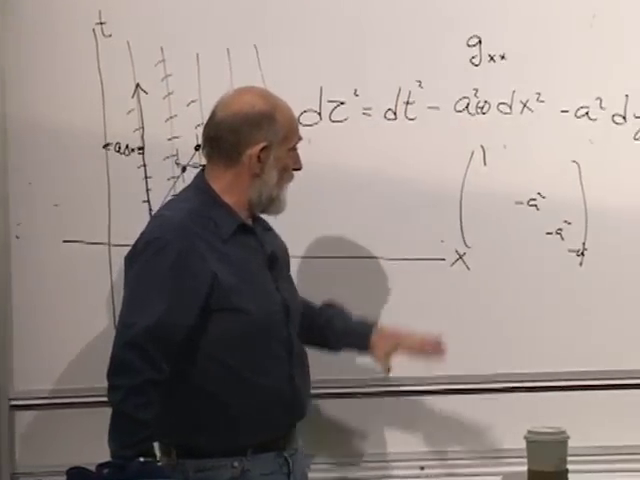
\includegraphics[width=0.82\textwidth]{lecture_01_figure_02.png}
\caption{膨脹的一維宇宙中的共動世界線，以及相應的時空間隔。}
\end{figure}

在三維空間中，同樣的形式可謹慎地推廣為\footnote{黑板上 00:56:38--00:58:51 附近的內容部分被遮住了。這個三維形式是根據講者將一維空間推廣到三維空間的說明，以及黑板上可見的對角形式而寫。}
\begin{equation}
d\tau^2=dt^2-a^2(t)\bigl(dx^2+dy^2+dz^2\bigr),
\end{equation}
度規為對角形式
\begin{equation}
g_{\mu\nu}=\mathrm{diag}\bigl(1,-a^2,-a^2,-a^2\bigr).
\end{equation}
非對角項為零：
\begin{equation}
g_{tx}=g_{ty}=g_{tz}=0.
\end{equation}

均勻性表示度規係數可以依賴時間，但不依賴空間位置。各向同性則表示三個空間方向的形式相同。

\begin{classroomqa}
\audiencequestion{我們不應該把 \(dx\) 視為距離嗎？}\lecturetimestamp{01:01:18}
\lecturerresponse{不。\(dx\)不是距離，\(a\,dx\)才是距離。\(dx\)只是標籤之間的間隔。可以這樣理解：想像有人在某個時刻穿過星系畫出座標網格，並要求網格隨星系移動。座標間隔依照定義保持固定，而物理距離則會改變。也可以把距離單位放進 \(x\)，而不是放進 \(a\)；這只是慣例。重要的是乘積 \(a\,dx\)。}
\end{classroomqa}

\begin{classroomqa}
\audiencequestion{\(dt^2\) 的度規係數等於 \(1\)。這也只是慣例嗎？}\lecturetimestamp{01:03:24}
\lecturerresponse{是的，單就這一點而言並沒有物理意義。如果該係數只依賴時間，就可以改變時間變數，讓它變成單純的 \(dt^2\)。同樣地，也可以選擇使用 \(c=1\) 的單位。這裡不屬於慣例的是：該係數不依賴位置，雖然它可以依賴時間。}
\end{classroomqa}

\begin{classroomqa}
\audiencequestion{如果把它代入愛因斯坦場方程，會得到什麼能量動量張量？}\lecturetimestamp{01:05:59}
\lecturerresponse{那是下一類問題，但屬於動力學，不在目前討論範圍內。可以把這個度規代入愛因斯坦方程，並問什麼樣的能量動量分布能使它成為一個解。這非常重要，但目前討論的是幾何，而不是動力學。}
\end{classroomqa}

\section{視界遮蔽了什麼}

只有在近似的意義下，我們才把大尺度宇宙視為均勻且各向同性。以恆星、行星，甚至單一星系的尺度來看，它顯然並不均勻；局部觀測也不會處處完全各向同性。

農田可以說明這種尺度依賴性。在某個尺度上，農田看起來很規則；尺度小得多時，顯然就不是如此；尺度大於整片農田時，它也不再顯得均勻。宇宙學也是如此。對許多星系取平均後，大尺度分布看起來大致均勻；在足夠小的尺度上則不然。

宇宙比我們看得見的部分更大，也比我們永遠能看見的部分更大。在實際可探測的尺度上，除了局部變化之外，宇宙是各向同性且均勻的。超出這個範圍，就沒有直接的觀測保證。

\begin{classroomqa}
\audiencequestion{你說我們永遠無法真正直接查明。這是否表示或許有間接查明的方法？}\lecturetimestamp{01:10:34}
\lecturerresponse{或許吧。如今多數人的看法是，宇宙在足夠大的尺度上並不均勻，我自己的猜測也一樣。但這個猜測永遠無法驗證：我不會贏，也不會輸。因為基於基本的物理原因，我們無法比現在看得遠太多。這就是視界的存在。}
\end{classroomqa}

\begin{classroomqa}
\audiencequestion{不能利用引力來尋找可觀測範圍以外的質量嗎？}\lecturetimestamp{01:11:53}
\lecturerresponse{不能。遙遠的質量可能只會使我們處於自由落體狀態。即使坐在封閉的房間裡，我們也處於太陽的引力場中並繞著它運行；但若看不到外面，就很難知道太陽就在那裡。只有潮汐力能揭示它的存在；如果引力源足夠遙遠，潮汐效應可能小到無法探測。}
\end{classroomqa}

因此，視界是直接知識的終極屏障。他甚至近乎確信地說，宇宙的體積至少是我們永遠能看見的區域的一千倍，至於這項說法的理由則留待稍後說明。

\section{有界而無邊界}

現在來看閉合幾何。無限直線是開放且無界的。線段則是有界的，意即其範圍有限。有界不表示存在邊界，而是指範圍有限。

有牆的立方體行不通。它違反均勻性，因為靠近牆的人和遠離牆的人並不等價；它也違反各向同性，因為即使是位於中心的人，朝不同方向看到的情況也不同。

圓或球的內部也不行。位於中心的人朝各個方向看到的情況相同，但這種對稱性只存在於一個特殊點。離開中心後，某個方向上的牆較近，另一個方向上的牆較遠。如此一來，一般位置的觀測者所處的空間既不均勻，也不具各向同性。

在極大的尺度上，工作假設是宇宙均勻且各向同性。這就是宇宙學原理。它很有用，但仍可能需要修正。

\begin{classroomqa}
\audiencequestion{處處各向同性是否代表均勻？}\lecturetimestamp{01:18:57}
\lecturerresponse{是。如果每位觀測者朝各個方向看到的情況都相同，就表示空間均勻。但反過來並不成立。均勻本身不代表各向同性。宇宙可以均勻，卻仍有優先方向；例如，若宇宙中充滿了指向同一方向的箭頭，就會如此。}
\end{classroomqa}

合適的有界模型是沒有任何特徵的球面。一個受限於球面上的二維生物，會發現每個位置在局部都和其他位置相同，各個方向也都彼此相同，儘管這個世界是有限的。這就是有界而無邊界。

\section{圓上的閉合一維宇宙}

為了讓代數保持簡單，把球面的例子簡化成一個空間維度：在圓上生活。在一維空間中，各向同性表示左與右等價；圓恰好具有這項特性。選一點作為 \(\theta=0\)。其他各點都以角座標 \(\theta\) 標記，角度以弧度為單位。緊鄰原點一側的點，可以用微小的負角描述，也可以用略小於 \(2\pi\) 的角描述。這種週期性是幾何的一部分。

圓上的居民能接觸到的是圓周，而不是外部的半徑或中心。他們可以沿著圓前進，直到回到原點，以此測量繞行一周的總距離。若把圓畫在周遭的平面上，也可以引入類似半徑的量；但那屬於嵌入圖像，不屬於居民所測量的內在幾何。

這裡的黑板圖很有用，因為角度標記和總周長都呈現在同一幅圖中。
\begin{figure}[H]
\centering
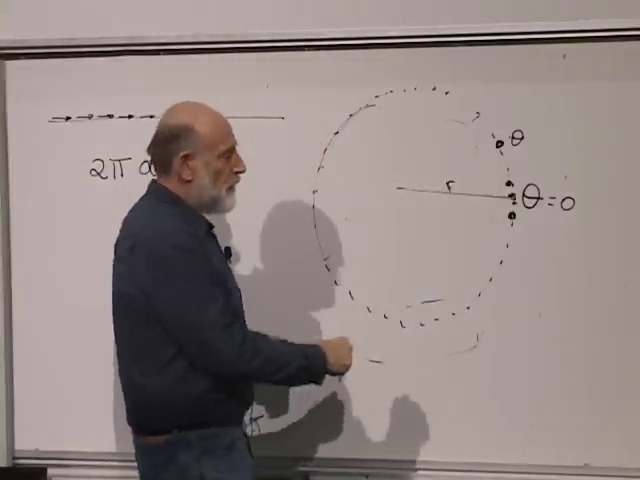
\includegraphics[width=0.82\textwidth]{lecture_01_figure_03.png}
\caption{閉合一維宇宙的角度描述，總周長為 \(2\pi a\)。}
\end{figure}

一種方便的慣例是\footnote{在 01：26：40--01：29：20，記號短暫地在兩種寫法之間切換：一種把整個圓周長直接當作標度因子，另一種則寫成 \(2\pi a\)。這裡採用後一種慣例，因為弧長公式使用的就是這種寫法。}
\begin{equation}
L=2\pi a,
\end{equation}
其中 \(L\) 是總周長。

對於微小的角間隔 \(\Delta\theta\)，物理距離為
\begin{equation}
d=a\,\Delta\theta.
\end{equation}
取無窮小極限可得
\begin{equation}
ds=a\,d\theta,
\end{equation}
因此
\begin{equation}
ds^2=a^2\,d\theta^2.
\end{equation}
這就是圓上的局部度規。

若 \(a\) 隨時間變化，閉合的一維宇宙就會膨脹或收縮。對固定的一對星系而言，
\begin{equation}
d(t)=a(t)\,\Delta\theta,
\end{equation}
因此
\begin{equation}
\dot d=\dot a\,\Delta\theta
      =\frac{\dot a}{a}\,d.
\end{equation}
這裡同樣適用哈勃定律，至少對於間距沒有大到使沿圓的另一側測量產生歧義的星系對而言。

時空度規變成
\begin{equation}
d\tau^2=dt^2-a^2(t)\,d\theta^2.
\end{equation}
若 \(a\) 為常數，時空圖像就是圓柱。若 \(a\propto t\)，圖像就是圓錐。若 \(a(t)\) 的變化較不規則，圖像就會像花瓶。

把圖像倒過來看，星系會彼此越來越接近。若圓周上有 \(360\) 個星系，到了較晚時期，它們會分布得很開；較早時則彼此非常接近，再往前推又會更近。最後，它們不再是彼此分離的星系；再往前推，甚至不再是彼此分離的原子。但空間中仍然沒有任何特殊點。

這就是在此模型中，對「大爆炸發生在哪裡？」這個問題最直接的回答。當 \(a(t)\to 0\) 時，每個間隔 \(a(t)\,\Delta\theta\) 都趨近於零。整個宇宙各處同時收縮。星系並不是從外部空間中的某個特定位置向外飛散；改變尺度的是幾何本身。就這個意義而言，答案是：無所不在。

\begin{classroomqa}
\audiencequestion{你說時空是彎曲的。如果時空是圓柱形，還會是彎曲的嗎？}\lecturetimestamp{01:38:04}
\lecturerresponse{不。如果是圓柱形，就不會是彎曲的。那是 \(a\) 隨時間保持常數的情形。它看起來是彎曲的，只是因為圖像畫在更高維的空間中。把圓柱剪開，就能不經拉伸而攤平。}
\end{classroomqa}

接著討論圓錐。若 \(a\propto t\)，時空圖像就是圓錐。遠離圓錐頂端的部分，在相同的內在意義上也是平坦的：可以把它展開成平面。頂端則不同；那裡是圓錐奇點。

接下來要討論球面宇宙的幾何，以及決定 \(a(t)\) 如何增長或縮小的動力學。

\chapter{牛頓宇宙學與弗里德曼方程}

上次我們談到了空間的度規。接下來要問的是動力學：尺度因子如何隨時間變化？我們先談一點幾何，再談牛頓宇宙學。這裡還不會從廣義相對論推導弗里德曼方程，而是從牛頓方程推導。

\section{均勻性、各向同性與隨時間變化的度規}

均勻性與各向同性是基本假設。如果宇宙均勻且各向同性，並且隨時間演化，那麼哈伯定律就一直成立。在任一固定時刻，退行速度與距離成正比，
\begin{equation}
v = H(t)\,d.
\end{equation}
這種正比關係是線性的。保持不變的不是時間，而是空間：在給定時刻，各處都適用同一個比例因子。

\begin{classroomqa}
\audiencequestion{你的意思是線性正比嗎？}\lecturetimestamp{00:02:06}
\lecturerresponse{是的。在固定時刻，退行速度與距離成線性正比。比例因子就是哈伯常數。一般而言，它會隨時間變化，但不會隨空間位置改變。}
\end{classroomqa}

所以「``哈伯常數''」這個說法容易引起誤解。它對空間位置而言是常數，對時間而言卻不是。

接下來自然會問：如果空間在膨脹，為什麼米尺也不跟著膨脹？答案是，把米尺結合在一起的力，遠強於原子尺度上任何與宇宙膨脹相關的效應。受束縛的物體仍維持束縛狀態。膨脹的是彼此距離足夠遠、互相束縛不強的物體之間的距離，例如相距甚遠的星系。

\begin{classroomqa}
\audiencequestion{測量用的尺也在膨脹，這會不會造成問題？}\lecturetimestamp{00:04:00}
\lecturerresponse{不會。測量用的尺並沒有膨脹，膨脹的是座標。把米尺結合在一起的力遠強於膨脹造成的效應，因此一般受束縛的物體不會隨著背景膨脹。相距足夠遠的星系確實會彼此分離，但米尺不會。}
\end{classroomqa}

甚至可以設想原子之間多了一點微弱的排斥效應，但這仍不足以把尺扯開。它只會稍微改變平衡間距，就像一點額外的拉力會稍微改變剛性彈簧的平衡位置。

\begin{classroomqa}
\audiencequestion{不過，你不能把它建模成作用在點與點之間的力，對嗎？否則它就會造成加速度。}\lecturetimestamp{00:05:29}
\lecturerresponse{可以設想原子之間存在一種微弱的額外作用力，但若它遠小於束縛力，就只會稍微改變平衡位置。單靠膨脹本身，不會產生一般的力定律。某些膨脹形式可以用力來建模，例如加速膨脹，但那是之後才要討論的問題。}
\end{classroomqa}

因此，適用的座標是嵌入在膨脹物質分布中的座標。沒有額外本動的星系，其座標值保持不變。隨時間改變的是座標間距與以公尺量度的物理距離之間的關係；這種關係由尺度因子\(a(t)\)表示。

在平坦空間中，空間度規可以寫成
\begin{equation}
ds^2 = a(t)^2\left(dx^2+dy^2+dz^2\right).
\end{equation}
這裡的\(a\)表示相隔一個單位座標距離的相鄰點之間的實際距離，以公尺為單位。如果宇宙膨脹，\(a\)就會隨時間變化。

要推廣到時空，可以從狹義相對論的形式出發
\begin{equation}
d\tau^2 = dt^2 - ds^2,
\end{equation}
並代入空間度規，得到
\begin{equation}
d\tau^2 = dt^2 - a(t)^2\left(dx^2+dy^2+dz^2\right).
\end{equation}
這些係數不隨空間位置改變，只隨時間變化。這就是均勻性在度規語言中的表述。對角度規的形式如下：
\begin{equation}
g_{\mu\nu}=\mathrm{diag}\!\left(1,-a(t)^2,-a(t)^2,-a(t)^2\right).
\end{equation}
\editorialnote{此處寫出的完整對角矩陣，依據的是00:14:33附近對度規張量的口頭描述。黑板畫面清楚顯示了線元素，但矩陣本身無法完整辨讀。}

沒有非對角項：沒有\(dx\,dy\)，沒有\(dx\,dt\)，也沒有其他混合項。這個度規幾乎和閔考斯基時空的度規一樣簡單。特別之處在於，空間尺度與時間之間的關係本身也隨時間變化。

\begin{figure}
\centering
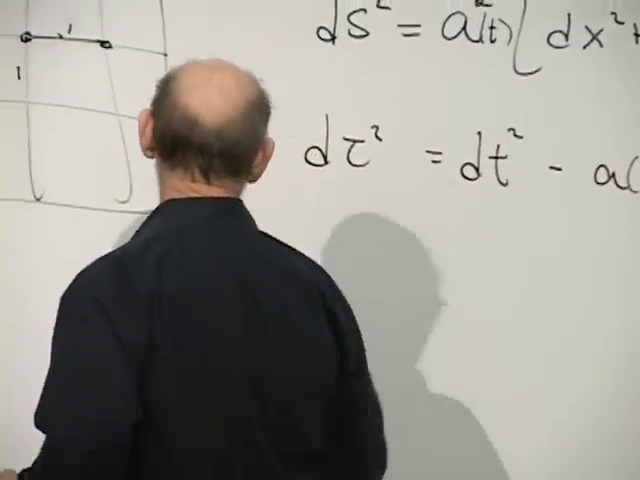
\includegraphics[width=0.62\textwidth]{lecture_02_figure_02.png}
\caption{共動座標網格示意圖，以及含時尺度因子的時空間隔。}
\end{figure}

圖示說明了重點。Alice 和 Bob 在共動座標中始終相隔一個單位，但隨時間經過，這一個座標單位所代表的公尺數愈來愈多。如果過去某個時刻的\(a(t)\)等於零，那麼所有物理距離都會是零，一切都會擠在一起。這就是為什麼\(a\to 0\)對應到無限密度。隨著\(a\)增大，宇宙會愈來愈稀薄。

這種度規形式並不適用於所有參考系；它適用於隨星系運動的參考系。

\begin{classroomqa}
\audiencequestion{那個方程裡的小\(t\)、\(a(t)\)，它的\(t\)是指什麼？}\lecturetimestamp{00:19:19}
\lecturerresponse{它是隨星系運動的時鐘所量到的時間。想像有一座宇宙時鐘工廠，製造出相同的時鐘，再把它們交給星系攜帶。在這個參考系中，時間變數正是這些時鐘所量到的時間。沿著星系的世界線，固有時等於這個座標時間。}
\end{classroomqa}

確實，沿著共動星系的世界線，
\begin{equation}
dx=dy=dz=0,
\end{equation}
所以
\begin{equation}
d\tau^2 = dt^2,
\end{equation}
因此
\begin{equation}
dt=d\tau.
\end{equation}

\begin{classroomqa}
\audiencequestion{有沒有能讓這種度規形式保持不變的變換？}\lecturetimestamp{00:23:08}
\lecturerresponse{旋轉可以，因為\(dx^2+dy^2+dz^2\)在旋轉下保持不變。但洛侖茲推進不會保留這種形式。物質本身選出了隨星系運動的參考系；在其他參考系中，宇宙看起來就不會是各向同性的。}
\end{classroomqa}

\section{重力場中的拋射體}

在把牛頓定律應用於整個宇宙之前，先回頭看一個較簡單的問題會有幫助：一個大質量\(M\)、一個小得多的質量\(m\)，以及一個初始的向外衝量。衝量作用之後，小質量只是在重力場中運動，依照牛頓定律演化。

在宇宙學的討論中，重要的不是完整的軌道問題，而是能量守恆。動能為
\begin{equation}
\frac{1}{2}mv^2.
\end{equation}

\begin{figure}
\centering
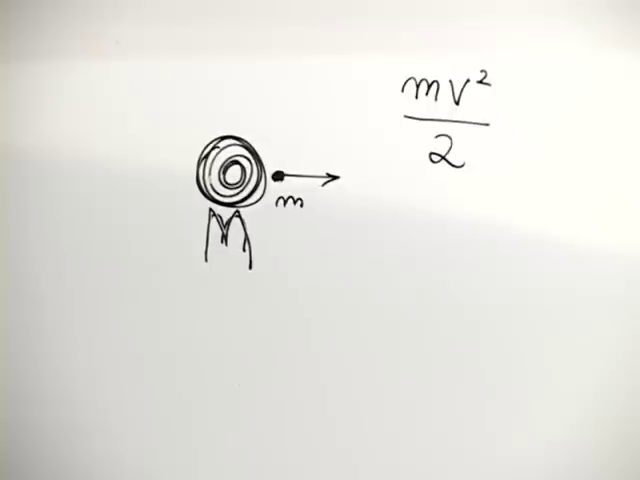
\includegraphics[width=0.42\textwidth]{lecture_02_figure_03.png}
\caption{向外運動的試驗質量與動能項\(\frac{1}{2}mv^2\)。}
\end{figure}

重力位能包含兩個質量的乘積、牛頓常數，以及分母中的一階距離。黑板上這些因子的排列順序是\(mMG/D\)，因此這裡最好沿用該順序：
\begin{equation}
-\frac{mMG}{D}.
\end{equation}
所以總能量為
\begin{equation}
\frac{1}{2}mv^2-\frac{mMG}{D}.
\end{equation}
能量守恆只表示，對正在討論的這個粒子而言，這個量不隨時間改變。不同粒子的能量可以不同。

\begin{figure}
\centering
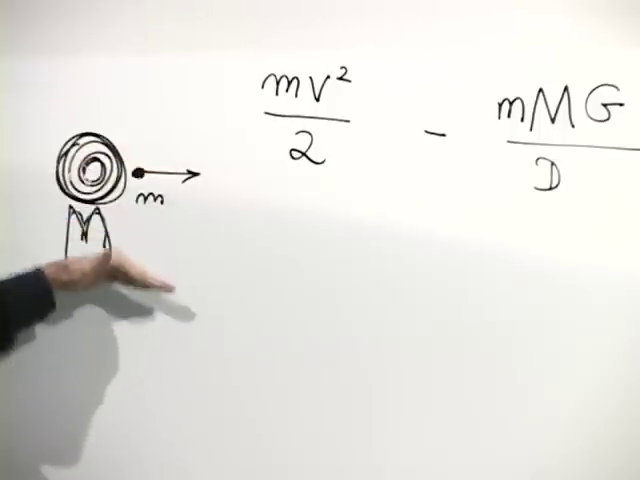
\includegraphics[width=0.62\textwidth]{lecture_02_figure_04.png}
\caption{徑向運動的試驗質量之牛頓總能量：動能減去重力位能。}
\end{figure}

負號很重要。重力位能是負的，因為重力具有吸引性。粒子愈靠近，位能就愈負；粒子移得愈遠，位能就愈不負。

\begin{classroomqa}
\audiencequestion{位能是隨距離增加而上升，不是下降嗎？}\lecturetimestamp{00:34:13}
\lecturerresponse{是的。先不管常數，看看\(1/D\)和\(-1/D\)的圖形。力會使物體朝位能降低的方向運動。因此，吸引力對應到倒過來的曲線\(-1/D\)；位能會隨距離增加而上升，粒子向內移動時則變得更負。}
\end{classroomqa}

\begin{figure}
\centering
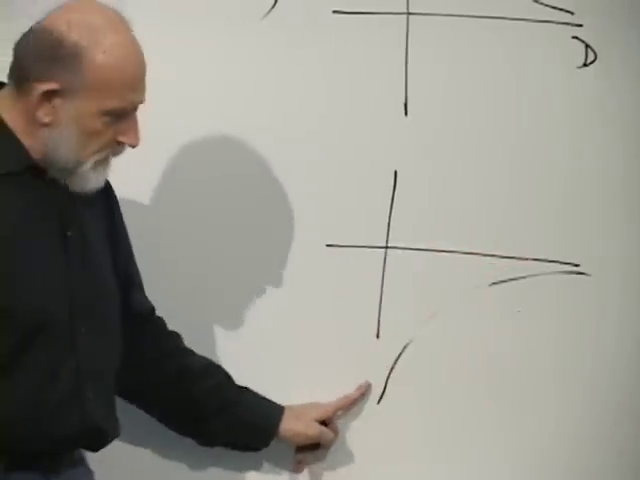
\includegraphics[width=0.46\textwidth]{lecture_02_figure_05.png}
\caption{比較\(1/D\)與\(-1/D\)的定性圖形，以說明重力位能的正負號。}
\end{figure}

\section{逃逸速度}

現在來分類各種可能性。能量可以是正、負或零，只有這三種情況。

\begin{itemize}
\item 能量為負時，粒子是受束縛的。若以太小的速度把它向上拋，它會上升、減速、折返，然後落回來。
\item 能量為正時，粒子會逃逸。重力起初會使它減速，但減速不足以讓它停下來；最後它會以非零的漸近向外速度遠離。
\item 能量恰好為零時，粒子正好達到逃逸速度。這是能否逃逸的臨界情況。
\end{itemize}

初始速度夠小時，一開始就是位能項占優勢，因此總能量為負。

\begin{figure}
\centering
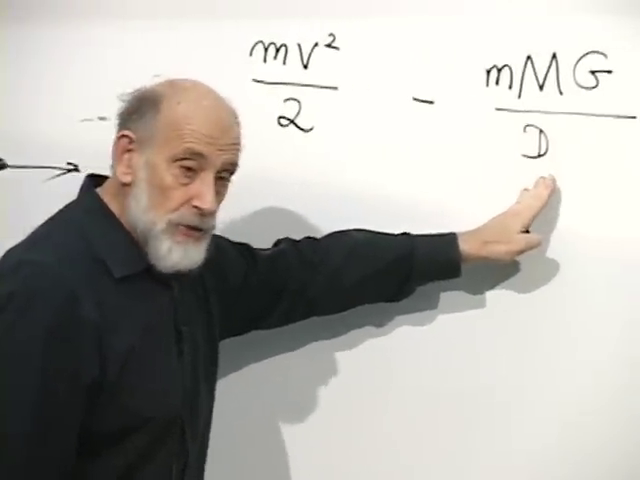
\includegraphics[width=0.62\textwidth]{lecture_02_figure_06.png}
\caption{向外速率較小時，負的位能項在總能量中占優勢。}
\end{figure}

在零能量的情況下，距離持續增加，但速率持續減小。粒子不可能在有限時間內停下來；如果真的停下來，它就會掉回去。因此距離沒有上限，而速度趨近於零。

這就是對宇宙學有用的直接類比。宇宙也可能有相同的演化方式。若初始向外的哈伯流夠強，所有物體都會彼此遠離；若不夠強，重力就會勝出，宇宙將發生大崩塌。兩者之間還有一個臨界情況，恰好類似逃逸速度。

\section{牛頓定理}

之所以能將宇宙學問題化簡，是因為平方反比定律適用的牛頓定理。

如果物質以某個中心為對稱中心呈球對稱分布，那麼對分布外的粒子而言，重力作用恰好等同於全部質量集中在中心。但這個定理更進一步：如果粒子位於分布內部，只有半徑較小處的質量會產生作用；半徑較大處的質量不會產生淨力。

這個定理最簡潔的情形是薄殼。完美的球殼對殼內任何位置的粒子都不產生重力，即使粒子不在中心也是如此。乍看之下或許令人驚訝，但這確實是\(1/r^2\)定律的結果。

\begin{classroomqa}
\audiencequestion{你剛才舉的例子裡，粒子穿越邊界時，力似乎不連續；這點是不是有些令人驚訝？}\lecturetimestamp{00:48:19}
\lecturerresponse{是的。對理想的無限薄球殼來說，這確實令人驚訝，而且是\(1/r^2\)力定律特有的結果。真實的球殼有厚度，因此力的變化會平滑一些；但理想薄殼的這個明確結果，正是牛頓定理令人驚奇的性質。}
\end{classroomqa}

用一幅圖來想像，這個定理就比較容易理解。把點質量換成點狀水源。在三維空間中，向外的流量會按\(1/r^2\)遞減。把這種水源連續地分布在球殼上。球殼外的流動，恰好就像所有水源都集中在中心；球殼內則不會有淨流動，因為中心沒有水源。重力定理背後也是相同的結構。

這裡的重點不是重新推導定理，而是運用它。

\section{將均勻宇宙化為單體問題}

現在回到宇宙學。取宇宙中的一小塊區域，其中充滿均勻分布的星系。如果方便，也可以把自己放在中心。這只是為了方便；任何人都可以說自己位於中心，而推導出的方程都應該相同。

選取一個位於\(x\)軸上、共動座標為\(x\)的星系。由於宇宙具有各向同性，選哪條軸都無關緊要。以\(x=0\)為球心，畫一個通過該星系的球面。根據牛頓定理，作用在該星系上的力，恰好等同於球內所有質量都集中在球心時的情況；球外的物質則沒有貢獻。

這個球會隨星系一起膨脹。它始終包含相同的星系，因此總質量也不變，雖然它的物理半徑會隨時間改變。

因此，該星系的運動遵循與拋射體相同類型的能量方程：
\begin{equation}
\frac{1}{2}mv^2-\frac{mMG}{D}=\text{constant}.
\end{equation}
這裡的\(M\)現在指膨脹球體內的質量，而不是前面簡單例子中的中心質量。接著，將方程乘以\(2\)並除以\(m\)，即可簡化代數式。常數除以\(m\)仍然只是常數，因此可以寫成
\begin{equation}
v^2-\frac{2MG}{D}=\text{constant}.
\end{equation}
同樣地，「``常數''」是指對這個特定星系而言，該量不隨時間改變。

現在把這個結果與尺度因子連結起來。到該星系的物理距離為
\begin{equation}
D=ax,
\end{equation}
因為\(x\)是固定的共動座標。它的速度為
\begin{equation}
v=\dot D=\dot a\,x.
\end{equation}

球內的質量等於密度乘以體積。若\(\rho\)表示質量密度，則
\begin{equation}
M=\frac{4\pi}{3}\rho D^3=\frac{4\pi}{3}\rho a^3x^3.
\end{equation}
代入能量方程可得
\begin{equation}
\dot a^2x^2-\frac{2G}{ax}\left(\frac{4\pi}{3}\rho a^3x^3\right)=\text{constant},
\end{equation}
也就是
\begin{equation}
\dot a^2x^2-\frac{8\pi G}{3}\rho a^2x^2=\text{constant}.
\end{equation}

左側兩項都正比於\(x^2\)，而左側其他量在各處都相同。因此右側也必須正比於\(x^2\)。這和稱它為常數並不矛盾：對每個固定的\(x\)而言，它不隨時間變化，但從一個星系到另一個星系，它仍可能隨\(x^2\)改變。這很合理，因為距離較遠的星系運動得比較快。

因此，約去共同因子\(x^2\)。剩下的常數現在不隨時間或空間改變。依照歷史上慣用的方式，把它寫成\(-k\)：
\begin{equation}
\dot a^2-\frac{8\pi G}{3}\rho a^2=-k.
\end{equation}
再除以\(a^2\)，得到
\begin{equation}
\left(\frac{\dot a}{a}\right)^2=\frac{8\pi G}{3}\rho-\frac{k}{a^2}.
\end{equation}

這就是著名的弗里德曼－羅伯遜－沃克方程，不過講課時也提到，這其實就是弗里德曼方程。符號的選法沿襲自歷史。寫成\(-k\)不表示\(k\)必須為正；\(k\)可以為正、為負或為零。在光速設為\(1\)的單位制中，\(k\)是無因次量。

\section{密度與物質主導的方程}

接下來自然要問：\(\rho\)是什麼？它不是常數。宇宙膨脹時，密度會降低。

要表示這種變化，可以在座標空間取一個單位立方體：沿\(x\)、\(y\)和\(z\)方向的邊長各為一個單位。由於立方體隨座標一起膨脹，裡面始終是相同的星系。因此，這個座標立方體內的質量固定不變。

\editorialnote{講課中在不同階段重複使用符號\(M\)。這裡以\(M_{\Box}\)表示單位座標立方體內的質量，藉此和前面提到的中心質量及球內質量區分。}

立方體的物理邊長是\(a\)，所以物理體積為\(a^3\)。因此
\begin{equation}
\rho=\frac{M_{\Box}}{a^3}.
\end{equation}
這是物質主導的情況：方程右側只包含普通非相對論性物質的密度。

\begin{classroomqa}
\audiencequestion{根據這個方程，哈伯常數是\(\rho\)的函數，所以它不是常數。}\lecturetimestamp{01:19:21}
\lecturerresponse{正是如此。哈伯常數不是常數。它取決於密度，而密度會隨時間變化。講課時甚至開玩笑說，期末考只要出一題就夠了：哈伯常數是常數嗎？}
\end{classroomqa}

將\(\rho=M_{\Box}/a^3\)代入弗里德曼方程，得到
\begin{equation}
\left(\frac{\dot a}{a}\right)^2=\frac{8\pi G M_{\Box}}{3a^3}-\frac{k}{a^2}.
\end{equation}

現在可以看出有哪些任意選擇：需要知道單位座標立方體內的質量，以及\(k\)的值。\(k\)的三種可能符號，分別對應拋射體問題中的三種能量情況。

\begin{itemize}
\item 若\(-k>0\)，能量相當於高於逃逸速度，宇宙會永遠膨脹。
\item 若\(-k<0\)，重力終將勝出，宇宙會重新坍縮。
\item 若\(k=0\)，宇宙恰好處於逃逸速度的臨界情況。
\end{itemize}

\begin{classroomqa}
\audiencequestion{若\(k=0\)呢？那麼兩個星系之間的速度會趨近於零嗎？}\lecturetimestamp{01:21:12}
\lecturerresponse{是的。在臨界情況下，速度會趨近於零，但距離仍然沒有上限。星系持續分離，只是速度愈來愈慢。如果它們真的在有限時間內停下來，就會掉回去。}
\end{classroomqa}

\section{臨界情況 \(k=0\)}

現在選擇最簡單的情況，也就是\(k=0\)。這正是逃逸速度的臨界情況；它之所以簡單，只是因為數學比較簡單。方程變成
\begin{equation}
\left(\frac{\dot a}{a}\right)^2=\frac{8\pi G M_{\Box}}{3a^3}.
\end{equation}

右側恆為正，從不等於零。因此\(\dot a/a\)不可能變為零。在這種情況下，宇宙不可能掉頭；它只能一直膨脹或一直收縮。這裡選擇膨脹分支。

現在猜測解具有冪次律的形式：
\begin{equation}
a(t)=ct^p.
\end{equation}
於是
\begin{equation}
\dot a = cp\,t^{p-1},
\end{equation}
因此
\begin{equation}
\frac{\dot a}{a}=\frac{p}{t}.
\end{equation}
代入微分方程，得到
\begin{equation}
\frac{p^2}{t^2}=\frac{8\pi G M_{\Box}}{3c^3t^{3p}}.
\end{equation}
要讓\(t\)的冪次相符，必須有
\begin{equation}
3p=2.
\end{equation}
所以
\begin{equation}
p=\frac{2}{3}.
\end{equation}
接著，常數必須滿足
\begin{equation}
\frac{4}{9}=\frac{8\pi G M_{\Box}}{3c^3},
\end{equation}
因此
\begin{equation}
c^3=6\pi G M_{\Box}.
\end{equation}
所以
\begin{equation}
a(t)=\left(6\pi G M_{\Box}\right)^{1/3}t^{2/3}.
\end{equation}

仍可能有一個加法形式的時間平移；把\(t\)換成\(t-t_0\)就能將它吸收。選擇時間原點，使\(t=0\)時\(a=0\)，剩下的常數便消失。

所以宇宙的膨脹尺度與時間的三分之二次方成正比，
\begin{equation}
a(t)\propto t^{2/3}.
\end{equation}
膨脹並非隨時間線性增加。線性成長相當於不加速的運動；這裡的膨脹則逐漸減慢。

若把公式往回推到\(t=0\)，尺度因子會降為零，密度則發散。\(a=0\)這種情況極端得難以想像。我們不知道物質在密度極高時會變成什麼樣子。真正的重點是，在宇宙早期的某個階段，一切都極度擁擠，原子、原子核和夸克全都擠在一起，處於極端高密度的狀態。

\section{哈伯常數與宇宙年齡}

在臨界模型中，
\begin{equation}
H(t)=\frac{\dot a}{a}=\frac{2}{3t}.
\end{equation}
所以哈伯常數約等於宇宙年齡的倒數：
\begin{equation}
t=\frac{2}{3H}.
\end{equation}
這是這項計算的一個主要成果。測量今天的哈伯常數，就能估算宇宙的年齡，至少可以回溯到牛頓模型不再適用之處。

引用的宇宙年齡約為\(13\)到\(14\)億年。文中也指出，\(k=0\)在觀測上相當符合實際：以文中引用的精度而言，尚未發現與\(k=0\)有顯著差異。

\begin{classroomqa}
\audiencequestion{我有點不太清楚\(M\)和\(a\)代表什麼。}\lecturetimestamp{01:39:16}
\lecturerresponse{兩者都帶有座標網格選擇所造成的任意性。改變基準立方體，其中的物質量會跟著改變，尺度因子的數值也會改變。具有物理意義的是密度\(M/a^3\)，或等價地，像\(a/M^{1/3}\)這樣不受網格選擇影響的組合。在\(k=0\)的解中，乘在\(t^{2/3}\)前面的未知常數會在\(\dot a/a\)中消去，因此年齡關係\(t=2/3H\)不取決於基準立方體內的質量。}
\end{classroomqa}

從解可以直接看出這個消去過程。若
\begin{equation}
a(t)=Ct^{2/3},
\end{equation}
則
\begin{equation}
\dot a=\frac{2}{3}Ct^{-1/3},
\end{equation}
因此
\begin{equation}
\frac{\dot a}{a}=\frac{2}{3t}.
\end{equation}
常數\(C\)完全消去。

\section{牛頓推導為何成立}

講到後面，問題就變成：為什麼牛頓推導能和相對論推導如此一致？

\begin{classroomqa}
\audiencequestion{這一切似乎都以宇宙為開放宇宙為前提。}\lecturetimestamp{01:45:44}
\lecturerresponse{目前的推導仍是牛頓式的，而牛頓物理意味著空間是平直的。至於 \(k\) 在空間幾何上的意義，留待下一講再說。屆時，\(k=0\)將對應平直空間，而其他符號則與彎曲的空間幾何相關。}
\end{classroomqa}

\begin{classroomqa}
\audiencequestion{很久以前，米尺的長度會不會取決於\(a\)？}\lecturetimestamp{01:47:53}
\lecturerresponse{在非常早期，物質會擁擠到分開的米尺根本無法存在；在那之前，它們也會被擠壓在一起。講課時也提醒我們，相對論不允許物體真正剛性：如果物體完全剛性，在一側推它，訊號就會瞬間傳到另一側，速度超過光速。}
\end{classroomqa}

\begin{classroomqa}
\audiencequestion{你認為牛頓方程和相對論方程為什麼會有這種巧合？}\lecturetimestamp{01:49:03}
\lecturerresponse{因為牛頓力學只用在足夠小的區域內。只要這個區域相較於整個宇宙的曲率半徑夠小，而且其中局部的哈伯速度遠低於光速，牛頓力學就是很好的近似。講課時把這件事比作研究地球上的草如何生長：不必考慮整個地球的曲率，也能理解局部的生長過程。}
\end{classroomqa}

這就是局部區域的推理方式。牛頓力學首先假設空間曲率對眼前的問題不重要，其次假設局部沒有任何物體以接近光速運動。在宇宙學中，這表示所選區域必須大到足以均勻，同時又要小到可以忽略曲率效應，並使哈伯速度維持在非相對論範圍內。

有了這個理解，牛頓計算就不是偶然得到的結果，而是某個方程在局部的近似；那個方程也可以用相對論的形式來表達。把曲率項移到左側，弗里德曼方程就變成
\begin{equation}
\left(\frac{\dot a}{a}\right)^2+\frac{k}{a^2}=\frac{8\pi G}{3}\rho.
\end{equation}
左側是幾何量，包含尺度因子，以及下一講會談到的空間曲率；右側則是能量密度。這正是廣義相對論所預期的方程形式。

下一講將討論曲率本身、愛因斯坦方程，以及相對論推導與牛頓推導之間的關係。

\chapter{弗里德曼膨脹、輻射與暗物質}

\section{基本宇宙學方程回顧}

在大於星系團的尺度上，宇宙可視為均勻的。選擇座標，使我們位於\(x=0\)，並將一個具代表性的星系，或單純視為隨哈伯流運動的假想粒子，置於\(x=1\)。依定義，它與我們的物理距離就是尺度因子\(a(t)\)。位於\(x=2\)的點距離我們\(2a(t)\)，依此類推。

\begin{figure}[ht]
\centering
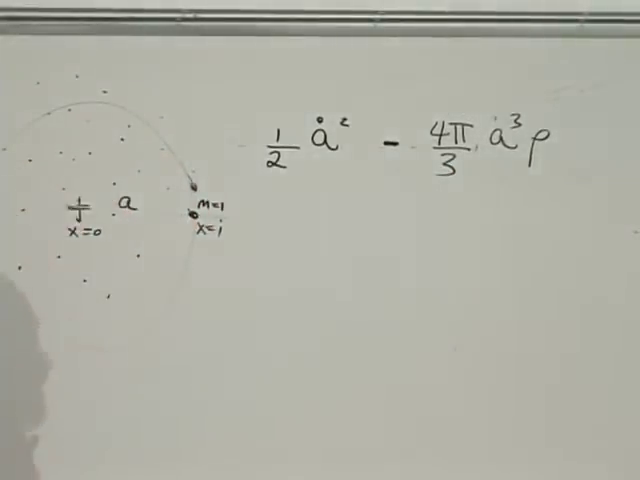
\includegraphics[width=0.78\textwidth]{lecture_03_figure_02.png}
\caption{以\(x=0\)為中心的均勻球體、位於\(x=1\)的共動星系，以及\(a(t)\)的牛頓力學能量平衡。}
\end{figure}

只有半徑為\(a(t)\)的球體內的物質，才會對位於\(x=1\)的粒子產生引力。令該粒子的質量為單位質量。它的動能為
\begin{equation}
\frac{1}{2}\dot a^2.
\end{equation}
球體內所含的質量為
\begin{equation}
M_{\mathrm{enc}}=\frac{4\pi}{3}a^3\rho,
\end{equation}
因此，引力位能為
\begin{equation}
-\frac{G M_{\mathrm{enc}}}{a}
=
-\frac{4\pi G}{3}a^2\rho.
\end{equation}
\editorialnote{在講課時間戳記00:05:30處，黑板上清楚寫出了動能項與依賴密度的位能項。此處列出的完整係數則是依據口頭推導補上。}

能量守恆給出
\begin{equation}
\frac{1}{2}\dot a^2-\frac{4\pi G}{3}a^2\rho=\text{const}.
\end{equation}
接著將常數記為\(-k\)；但要留意，只有將方程乘以\(2\)後，這個記號才符合標準正規化。在標準形式中，
\begin{equation}
\dot a^2=\frac{8\pi G}{3}a^2\rho-k,
\end{equation}
再除以\(a^2\)，得到
\begin{equation}
\left(\frac{\dot a}{a}\right)^2=\frac{8\pi G}{3}\rho-\frac{k}{a^2}.
\end{equation}
這就是本討論一貫使用的弗里德曼方程形式。

\begin{figure}[ht]
\centering
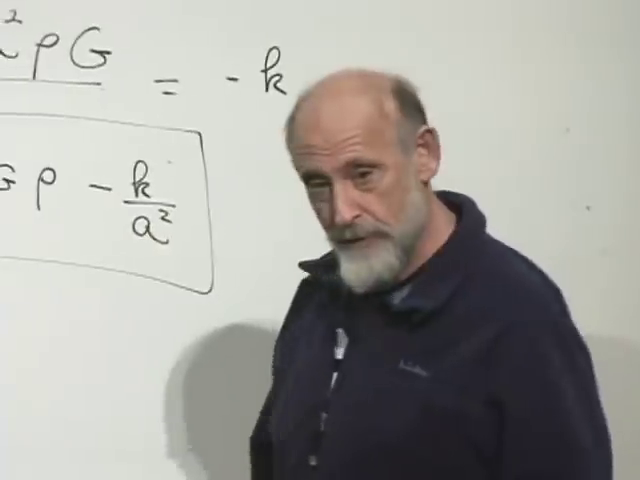
\includegraphics[width=0.56\textwidth]{lecture_03_figure_03.png}
\caption{弗里德曼方程中單獨標示出的曲率項\(-k/a^2\)。}
\end{figure}

觀測顯示，曲率項非常接近零；在這個層次上，將它忽略是相當好的近似。它確實代表空間曲率，但觀測到的效應太小，甚至無法判定曲率的正負。

同一個方程也可以從廣義相對論導出。示意而言，愛因斯坦方程的時間—時間分量為
\begin{equation}
R_{00}-\frac{1}{2}g_{00}R \propto T_{00}.
\end{equation}
\editorialnote{此處只列出張量結構，未列精確的整體數值係數。}
對於膨脹中的均勻度規，幾何側會產生\(\dot a/a\)與\(k/a^2\)的組合，物質側則是能量密度。就目前的討論而言，牛頓力學的論證與愛因斯坦方程描述的是同一件事。

這也改變了\(\rho\)的意義。從這裡開始，最好把\(\rho\)稱為能量密度。對共動參考系中緩慢運動的物質而言，它就是靜止能量密度。

\section{物質主導時期}

現在假設能量密度來自靜止於共動參考系中的物質。取一個座標邊長為一單位的立方體，其物理邊長為\(a(t)\)，因此物理體積為\(a^3(t)\)。若這個共動立方體內的質能為\(M\)，且物質隨著流動而不穿越立方體邊界，則
\begin{equation}
\rho_m=\frac{M}{a^3}.
\end{equation}

這就是物質主導的情形。在這個理想化模型中，粒子靜止於盒中，因此溫度視為零，壓力也視為零。要有壓力，粒子就必須穿越盒子的邊界。

令\(k\approx 0\)，方程便成為
\begin{equation}
\left(\frac{\dot a}{a}\right)^2=\frac{8\pi G}{3}\frac{M}{a^3}.
\end{equation}
試取冪次形式
\begin{equation}
a(t)=Ct^p.
\end{equation}
則
\begin{equation}
\frac{\dot a}{a}=\frac{p}{t},
\end{equation}
因此左側正比於\(t^{-2}\)，右側正比於\(t^{-3p}\)。比較冪次可得
\begin{equation}
3p=2,
\qquad
p=\frac{2}{3}.
\end{equation}
所以
\begin{equation}
a(t)\propto t^{2/3}.
\end{equation}
再比較係數可得
\begin{equation}
C^3=6\pi G M.
\end{equation}

這個解的重點在於冪次律。物質主導的宇宙，其膨脹與時間的三分之二次方成正比，而非線性正比。這個定律描述一段漫長的中間時期，約從大爆炸後\(10^5\)年開始，延續到幾十億年後。如今的宇宙並非嚴格由物質主導，因為暗能量目前占主導地位；不過，普通物質的行為以及宇宙歷史中很長的一段時期，都可以用這個模型描述。

\section{輻射主導時期}

在更早的時期，能量密度由輻射主導。原因很簡單：宇宙中有極大量的光子，每個質子大約對應\(10^9\)個光子；宇宙被壓縮時，這些光子的能量會升高。

光子沒有靜止質量，但有能量。其能量為
\begin{equation}
E_\gamma=h\nu=\frac{hc}{\lambda}.
\end{equation}
關鍵假設是，宇宙膨脹時，光子的波長也隨之伸長：
\begin{equation}
\lambda\propto a.
\end{equation}
盒中的波可以幫助理解這一點：盒子變大，波模的波長也隨盒子變長。這裡將相同的想法應用於膨脹中的宇宙。

由於\(\lambda\propto a\)，每個光子的能量正比於
\begin{equation}
E_\gamma\propto a^{-1}.
\end{equation}
再取一個共動的單位盒子。光子會進出盒子，但平均而言，盒內光子數維持不變。因此，盒內光子的總能量也正比於\(a^{-1}\)。再除以物理體積\(a^3\)，輻射能量密度便正比於
\begin{equation}
\rho_r\propto a^{-4}.
\end{equation}

多出的\(a^{-1}\)因子就是兩者的差異所在。宇宙膨脹會稀釋物質。輻射除了因膨脹而稀釋，每個光子還會因紅移而損失能量。

因此，輻射主導宇宙的弗里德曼方程為
\begin{equation}
\left(\frac{\dot a}{a}\right)^2=\frac{8\pi G}{3}\frac{M_r}{a^4}.
\end{equation}
\editorialnote{口頭講解中再次使用符號\(M\)表示這個新常數。此處加上\(r\)下標，只是為了與物質主導的情形區別。}

使用相同的試探形式\(a(t)=Ct^p\)。左側同樣正比於\(t^{-2}\)，右側則正比於\(t^{-4p}\)。比較冪次可得
\begin{equation}
4p=2,
\qquad
p=\frac{1}{2}.
\end{equation}
因此
\begin{equation}
a(t)\propto t^{1/2}.
\end{equation}
再比較係數可得
\begin{equation}
C^4=\frac{32\pi G}{3}M_r.
\end{equation}

\begin{classroomqa}
\lecturetimestamp{00:35:41}
\audiencequestion{為什麼裡面會有\(G\)？}
\lecturerresponse{因為產生引力效應的是能量密度，而不只是靜止質量。對緩慢運動的物質而言，這項差異很容易被忽略；但光子讓我們無法忽視這一點：光子沒有靜止質量，仍然會產生引力。}
\end{classroomqa}

裝滿輻射的盒子可以具體說明這一點。推動一個裝滿光子的盒子。盒子一旦加速，朝光子移動的盒壁受到的撞擊會比遠離光子的盒壁更強，因此必須更用力推，才能克服輻射壓。於是盒子有了額外的慣性；根據等效原理，這份額外慣性也代表額外的引力質量。這就是此處用來說明能量會產生引力的「光子盒」論證。

\begin{classroomqa}
\lecturetimestamp{00:38:11}
\audiencequestion{這兩個方程是否有任何一個存在\(a\)隨時間減小的解？}
\lecturerresponse{有。若把曲率項\(k/a^2\)加回去，就會有先膨脹再收縮的解。我們的宇宙看來並非如此演化，但方程確實允許這種解。}
\end{classroomqa}

\begin{classroomqa}
\lecturetimestamp{00:38:44}
\audiencequestion{那能量守恆呢？}
\lecturerresponse{若把\(k\)項加回去，並將方程乘回\(a^2\)，宇宙學方程正好就是守恆定律。方程一側的物質或輻射只是整體收支的一部分。膨脹也帶來動能與引力位能的部分，而總能量收支守恆。}
\end{classroomqa}

\section{物質與輻射並存}

真實的宇宙同時包含物質與輻射，兩者的密度隨尺度因子的變化不同：
\begin{equation}
\rho_m\propto a^{-3},
\qquad
\rho_r\propto a^{-4}.
\end{equation}
因此，\(a\)很小時由輻射主導；\(a\)很大時則由物質主導。往回追溯，早期宇宙必定由輻射主導。

\begin{figure}[ht]
\centering
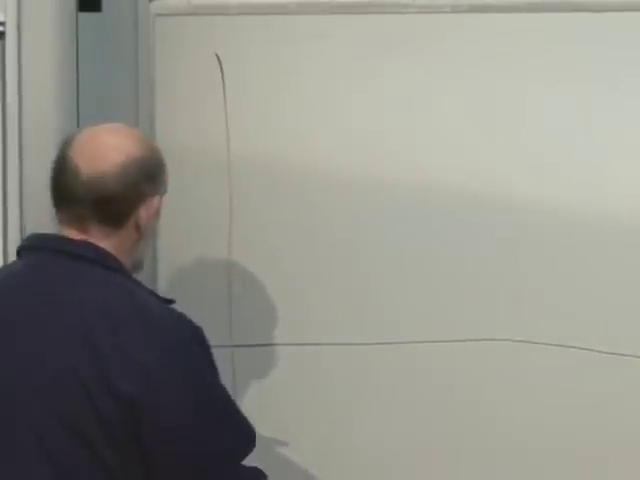
\includegraphics[width=0.68\textwidth]{lecture_03_figure_05.png}
\caption{比較物質與輻射能量密度隨尺度因子變化的座標軸。}
\end{figure}

\editorialnote{在講課時間戳記00：44：45處，黑板上只畫出了比較圖起始處的座標軸。緊接著討論的物質與輻射曲線只在正文中描述，並未在此重新繪出。}

物質曲線依\(a^{-3}\)的規律下降，輻射曲線則依\(a^{-4}\)的規律下降。當\(a\to 0\)時，兩者都發散，但輻射曲線在該處上升得更快，因此兩條曲線會在某個相等時的尺度因子處相交。粗略估計，這個轉變發生在大約\(10^4\)年後，或許還要稍久一些。

也可以用\(a(t)\)對\(t\)的圖來呈現同一件事。早期的膨脹行為類似\(t^{1/2}\)，後期則類似\(t^{2/3}\)。這項變化不是突然跳變，而是在相對狹窄的時間範圍內連續過渡。

\begin{classroomqa}
\lecturetimestamp{00:44:04}
\audiencequestion{隨著宇宙變老，冪次\(p\)會從\(1/2\)連續變為\(2/3\)嗎？}
\lecturerresponse{會。它不會突然跳變，而是連續改變，只是變化集中在相當狹窄的時間範圍內。}
\end{classroomqa}

\section{溫度、複合與最後散射}

接下來考慮溫度。若典型光子的能量正比於\(a^{-1}\)，輻射場的溫度也同樣如此：
\begin{equation}
T\propto a^{-1}.
\end{equation}
若\(a\)加倍，溫度就會減半。

取目前的光子溫度約為\(3\,\mathrm K\)，電離溫度約為\(3000\,\mathrm K\)，大致相當於太陽表面的溫度。則
\begin{equation}
\frac{a_{\mathrm{today}}}{a_{\mathrm{ion}}}\sim 10^3.
\end{equation}
使用晚期物質主導時期的定律\(a\propto t^{2/3}\)，
\begin{equation}
\left(\frac{t_{\mathrm{today}}}{t_{\mathrm{ion}}}\right)^{2/3}\sim 10^3,
\end{equation}
因此
\begin{equation}
\frac{t_{\mathrm{today}}}{t_{\mathrm{ion}}}\sim 1000^{3/2}\sim 3\times 10^4.
\end{equation}
以這項估算的精度，取宇宙年齡為\(10^{10}\)年，可得
\begin{equation}
t_{\mathrm{ion}}\sim 3\times 10^5\ \mathrm{years}.
\end{equation}

這是氫與氦不再完全電離的時期。在此之前，宇宙是高溫電漿。為什麼電漿不透明？因為自由電荷會強烈響應電磁波。電場驅使電荷來回運動，使介質表現得像導體；而導體是不透明的。這就是此處與太陽表面相比的原因。

宇宙冷卻到電子能與原子核複合後，普通的中性原子便形成，宇宙也變得透明許多。這項轉變並非在某個瞬間完成，而是發生於一段模糊的時間區間。不過對宇宙學而言，這段區間仍界定得夠清楚，因此稱為最後散射面。

向外看，就是回望過去。鄰近星系呈現的是較近的過去；更遙遠的星系則呈現更早的時期。距離夠遠時，每一條視線都會抵達宇宙仍處於電離、不透明狀態的時期。電磁輻射無法讓我們看到更早的宇宙。

原則上，其他信使可以探測更早的時期。中微子不帶電，會更早退耦。引力子若有朝一日能被觀測到，則會來自更早的時期。然而，正是讓它們能穿過早期電漿的微弱交互作用，也使它們極難探測。

如果宇宙曾經在各個方向上都像太陽表面一樣灼熱，為什麼天空沒有亮得令人目眩？因為最後散射面正在遠離我們，從那裡抵達的光子已經紅移了約\(10^3\)倍，恰好相當於\(3000\,\mathrm K\)與\(3\,\mathrm K\)之間的溫度比。抵達我們的是微波輻射，而不是可見光中的陽光。

\begin{classroomqa}
\lecturetimestamp{01:03:51}
\audiencequestion{所以我們的望遠鏡無法看到大約\(300{,}000\)年以前的宇宙嗎？}
\lecturerresponse{電磁望遠鏡無法做到。在那之前，宇宙處於電離且不透明的狀態。其他信使至少原則上能探測更早的時期。}
\end{classroomqa}

\begin{classroomqa}
\lecturetimestamp{01:08:43}
\audiencequestion{你說光子的溫度，是指具有該峰值輻射的黑體溫度。但這和波長並非線性關係，對吧？}
\lecturerresponse{沒錯。溫度本質上代表典型光子的能量，因此對光子而言，溫度與波長成反比。\(T^4\)定律描述的是能量密度，而非單一光子的能量；它結合了每個光子的能量與單位體積內的光子數，而光子數密度正比於\(T^3\)。}
\end{classroomqa}

因此
\begin{equation}
n_\gamma\propto T^3,
\qquad
\rho_\gamma\propto T^4.
\end{equation}

\section{從旋轉曲線推知暗物質}

暗物質的證據來自星系旋轉曲線。它並非從大尺度的弗里德曼方程推知，而是從星系尺度的天文觀測推知。

從最簡單的牛頓力學問題開始：質量為\(m\)的輕質物體，以\(M\)為中心質量，在半徑\(r\)處繞行。引力大小為
\begin{equation}
\frac{GMm}{r^2},
\end{equation}
向心加速度則為\(v^2/r\)。牛頓定律給出
\begin{equation}
m\frac{v^2}{r}=\frac{GMm}{r^2}.
\end{equation}
約去\(m\)，再乘以\(r\)，可得
\begin{equation}
v(r)=\sqrt{\frac{GM}{r}}.
\end{equation}
所以，若引力質量集中在中心附近，軌道速度便會依\(r^{-1/2}\)的規律下降。

如果質量分布跟著光的分布，這正是預期的結果。星系中大部分可見物質位於核心附近，因此外圍恆星的運動應類似外太陽系中的行星。天文學家測量鄰近星系兩側的多普勒位移差異，以推知軌道速度：先扣除整個星系的退行運動，再比較朝我們運動的一側與遠離我們的一側。觀測到的軌道速度在很大的半徑範圍內仍大致不變。

因此，將中心質量\(M\)換成半徑內的總質量\(M(r)\)：
\begin{equation}
\frac{v^2}{r}=\frac{G M(r)}{r^2}.
\end{equation}
若\(v(r)\)近似不變，則
\begin{equation}
M(r)\propto r.
\end{equation}
換句話說，即使可見光不再增加，引力質量仍會隨半徑持續增加。

現在依照此處為求簡化所採用的假設，令質量分布大致呈球對稱。則
\begin{equation}
M(R)=\int_0^R 4\pi r^2\rho(r)\,dr.
\end{equation}
若\(M(R)\propto R\)，對\(R\)微分可得
\begin{equation}
4\pi R^2\rho(R)\propto 1,
\end{equation}
因此
\begin{equation}
\rho(r)\propto \frac{1}{r^2}.
\end{equation}

\begin{classroomqa}
\lecturetimestamp{01:28:18}
\audiencequestion{看起來密度應該正比於\(1/r^2\)。這是有原因的嗎？}
\lecturerresponse{從觀測到的平坦旋轉曲線可推得\(M(R)\propto R\)，再微分便得到\(\rho(r)\propto 1/r^2\)。除此之外，此處並未提出簡單的第一原理解釋；詳細模擬在這方面發揮了很大作用。}
\end{classroomqa}

可以確定的是，星系的引力質量遠大於僅從發光物質推算出的質量，大約多出數倍；依此處採用的估計，則約多出一個數量級。可見星系位於大得多的暗物質暈之中。

為什麼普通氣體不會維持在這種稀薄狀態？原因是耗散。氣體雲會收縮，是因為碰撞、類似摩擦的過程以及輻射讓它能量逐漸流失。暗物質顯然不會顯著輻射，而且幾乎不發生碰撞。引力可以將它向內拉，並把位能轉換成動能；但若沒有有效的耗散，它就不會坍縮成普通物質形成的緻密發光結構。維持暗物質暈延展的，是動能。

接著謹慎地討論了幾種替代可能。中微子的速度太快，無法在星系尺度上形成這樣的結構。由普通氫構成的暗物質暈會嚴重影響早期宇宙的核合成。由普通物質形成的黑洞也有問題，因為這代表早期宇宙中的普通物質過多，並會帶來引力透鏡方面的問題；此處的討論並未進一步主張其他結論。

暗物質暈並非薄殼或環面，而是一個近似球形、密度不均的球體：中心較密，往外逐漸變稀。

\begin{classroomqa}
\lecturetimestamp{01:53:12}
\audiencequestion{你說的是子彈星系團嗎？}
\lecturerresponse{是。X射線氣體顯示普通物質的分布，引力透鏡則顯示總引力質量的分布。在這次碰撞中，兩者分離了。這是暗物質確實存在的有力證據，而非僅僅修改與可見物質相關的引力理論。}
\end{classroomqa}

這就是最後一項觀測重點。人們對暗物質本質的細節所知甚少，但此處的論述不需要引入激進的新原理。一種保守的可能性是，自然界中還有尚未辨識出的弱交互作用粒子。
\chapter{視界、狀態方程與真空能}

\section{優選參考系、超光速退行與視界}

宇宙微波背景輻射確實標示出一個特殊參考系。在這個參考系中，該輻射看起來是各向同性的；附近星系平均而言也處於靜止。如果我們相對於背景運動，前進方向上的光子會因多普勒效應而移向較高能量，後退方向上的光子則移向較低能量。優選參考系就是微波背景看起來各向同性的參考系；平均而言，本地星系也在這個參考系中靜止。

\begin{classroomqa}
\lecturetimestamp{00:00:25}
\audiencequestion{宇宙輻射的表觀波長是否取決於觀測者的運動？這是否意味著存在優選參考系？}
\lecturerresponse{是的。相對於微波背景運動會產生多普勒各向異性，因此存在一個優選的宇宙學參考系，也就是微波背景看起來各向同性的參考系。平均而言，本地星系也在這個參考系中靜止。}
\end{classroomqa}

第二個問題關於退行速度。哈伯定律指出，足夠遙遠的星系彼此遠離的速度符合
\begin{equation}
v = H d .
\end{equation}
當 \(d\) 夠大時，這個退行速度會超過光速。這並不違反相對論，因為相對論的限制是局部的：一個物體不能在我們眼前以超光速掠過另一個物體。遙遠星系的情形，描述的是相距甚遠的地方之間的幾何關係。

\begin{classroomqa}
\lecturetimestamp{00:04:48}
\audiencequestion{兩個星系的相對速度能否大於 \(c\)？}
\lecturerresponse{可以，只要它們相距夠遠。哈伯退行速度可以超過光速而不違反局部相對論；退行速度達到 \(c\) 的地方就是視界。}
\end{classroomqa}

退行速度一旦達到光速，朝我們傳來的訊號就不再能縮短與我們之間的距離。光線在局部仍以極限速度前進，但它必須追上的距離增長得太快。

\begin{classroomqa}
\lecturetimestamp{00:07:03}
\audiencequestion{反方向發出的光線，難道不還是會朝我們前進嗎？}
\lecturerresponse{在局部確實如此，但空間膨脹的速度超過了光線追上我們的速度。光線相對於附近位置以極限速度前進，但回到我們這裡的總距離仍持續增加。}
\end{classroomqa}

\section{膨脹度規與直線類比}

一個有用的圖像是一維直線。想像一條由原子構成的線。若拉伸一條普通材料線，它最後會斷裂。現在改變這個圖像：每當相鄰原子相距太遠，就在它們之間插入另一個原子。這條線持續變長，但其局部性質不會因此變得稀疏。

\begin{figure}
\centering
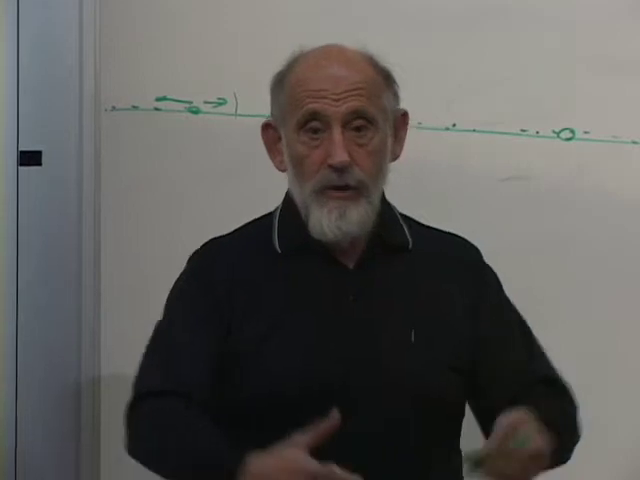
\includegraphics[width=0.60\textwidth]{lecture_04_figure_02.png}
\caption{用來描繪膨脹度規的一維直線。}
\end{figure}

在這個圖像中，局部仍有一個訊號速度上限，就像普通直線上的聲音也有速度上限。這條規則適用於局部：相對於附近的位置，擾動不能超過該速度。然而，如果直線夠長，而且新位置插入得夠快，距離夠遠的部分就會退行得太快，使訊號永遠無法返回。

因此，狹義相對論的速度合成定律只說明了部分情況。它適用於局部，也就是觀測者在同一位置彼此經過時。對於膨脹幾何中相距遙遠的星系，這並不是合適的描述方式。

\begin{classroomqa}
\lecturetimestamp{00:09:42}
\audiencequestion{在這種情況下，通常的相對論速度合成定律仍然適用嗎？}
\lecturerresponse{在局部、同一位置上，適用。如果觀測者依序彼此經過，通常的狹義相對論規則就適用。但要描述相距遙遠、退行速度超過 \(c\) 的情況，就不能用這種方式；必須回到膨脹空間的幾何。}
\end{classroomqa}

同一個圖像也能簡單說明紅移。在直線上畫一道波。直線膨脹時，波長也隨之伸長。在膨脹幾何中，這不只是形象化的說法；膨脹時空中的波動方程確實會導出波長伸長。

\begin{classroomqa}
\lecturetimestamp{00:14:42}
\audiencequestion{波隨著宇宙膨脹而伸長，這是理論推論、觀測結果，還是兩者皆是？}
\lecturerresponse{這是波在膨脹時空中傳播的理論推論，也有天文觀測支持。}
\end{classroomqa}

這個圖像不是橡皮筋。橡皮筋拉伸時會變細；生活在這種介質中的人會觀察到局部性質改變。這裡的局部性質保持不變，增長的是整體距離尺度。

\section{最後散射與可觀測宇宙}

視界是退行速度達到光速的地方。最後散射面位於視界稍內側。從視界發出的訊號會被無限紅移；最後散射輻射的紅移則極大，但仍有限。

\begin{classroomqa}
\lecturetimestamp{00:17:53}
\audiencequestion{超光速退行、最後散射面與可觀測宇宙之間有什麼關係？}
\lecturerresponse{視界是退行速度達到光速的地方。最後散射面位於視界稍內側，因為其紅移極大但仍有限。就實際而言，它標示了可觀測宇宙的邊界。}
\end{classroomqa}

最後散射輻射的紅移大約是 \(10^3\) 倍。這個數值已經非常大，因此在許多情況下，最後散射面都非常接近視界。可觀測宇宙是光能夠從中傳到我們這裡的那部分宇宙。

在晚期，膨脹會趨近真空能主導的狀態。此時哈伯參數趨於常數，視界則趨近固定大小；星系和微波輻射也會逐漸從視野中消失。

\begin{classroomqa}
\lecturetimestamp{00:22:43}
\audiencequestion{既然 \(H\) 會隨時間變化，視界距離也會變化嗎？微波背景最終會消失嗎？}
\lecturerresponse{在晚期，\(H\) 會趨於常數，因此視界會趨近固定距離。微波背景會持續伸長、冷卻並逐漸變得不可見。遙遠星系也會越過視界，從視野中消失。}
\end{classroomqa}

只有已受引力束縛的結構會繼續留在可觀測範圍內。太陽系不會飛散，星系也不會飛散，但大尺度宇宙會變成一座孤島。

\section{基本膨脹方程與三種組分}

現在來看基本膨脹方程：
\begin{equation}
\left(\frac{\dot a}{a}\right)^2 = \frac{8\pi G}{3}\rho ,
\qquad c=1 .
\end{equation}
其中 \(a(t)\) 是尺度因子，\(\rho\) 是總能量密度。

\begin{figure}
\centering
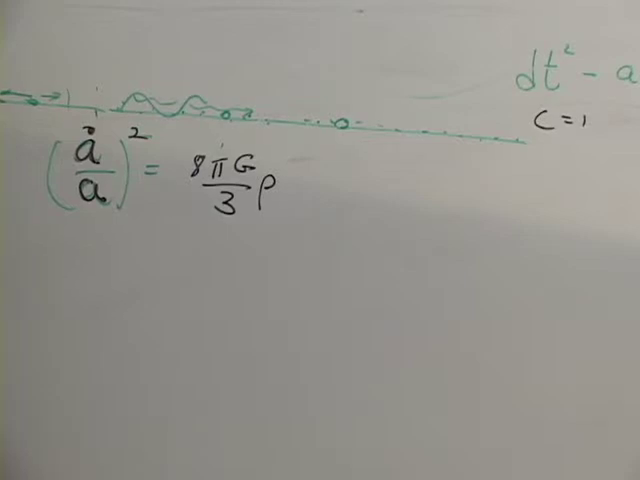
\includegraphics[width=0.74\textwidth]{lecture_04_figure_03.png}
\caption{基本膨脹方程與一維直線類比。}
\end{figure}

有三種組分在動力學上相當重要。

對物質而言，
\begin{equation}
\rho=\frac{\text{const.}}{a^3},
\qquad
a(t)\sim t^{2/3}.
\end{equation}
這描述有質量的物體隨整體膨脹運動，並且在共動參考系中基本上處於靜止的情況。

對輻射而言，
\begin{equation}
\rho=\frac{\text{const.}}{a^4},
\qquad
a(t)\sim t^{1/2}.
\end{equation}
多出的 \(a\) 次方來自宇宙膨脹時每個光子的紅移。

此外還有
\begin{equation}
\rho_0=\text{constant},
\end{equation}
真空能，也稱為暗能量；若不計傳統約定中的數值因子，它也稱為宇宙學常數。這種組分完全不會稀釋。

下一步是把能量密度和壓力聯繫起來。

\section{輻射壓力與冷物質}

先從輻射談起。考慮一個一維盒子，也就是長度為 \(L\) 的線段，裡面有光子來回反射。在一維中，力和壓力實際上是同一回事。

取一個動量大小為 \(p\) 的光子。它從盒壁反射時，動量的變化量為
\begin{equation}
\Delta p = 2p.
\end{equation}
它與同一面盒壁連續兩次碰撞之間的時間為
\begin{equation}
\Delta t = \frac{2L}{c}.
\end{equation}
因此，作用在盒壁上的平均力為
\begin{equation}
F=\frac{\Delta p}{\Delta t}=\frac{pc}{L}.
\end{equation}
對光子而言，
\begin{equation}
E=pc,
\end{equation}
所以
\begin{equation}
F=\frac{E}{L}.
\end{equation}
能量除以長度就是一維能量密度。在這個一維情況下，
\begin{equation}
P=\rho .
\end{equation}

有許多光子時，取平均後仍得到相同的關係。總力就是每單位長度的總能量。

現在來看三維情況。如果所有光子都只沿一個軸向運動，它們就只會對一對盒面施加壓力，而不會對其他盒面施壓。這個假設刻意設得不正確，但能立刻看出需要修正之處。在各向同性的光子氣體中，動量分布於各個方向。平均而言，能量密度的三分之一貢獻給每個壓力分量。結果是
\begin{equation}
P=\frac{\rho}{3}.
\end{equation}

冷物質的情況則不同。取一個共動盒子，也就是隨宇宙流動的一小塊區域。盒中的粒子帶有能量，但若它們相對於盒子靜止，就不會撞擊盒壁。因此壓力為
\begin{equation}
P=0.
\end{equation}

\begin{figure}
\centering
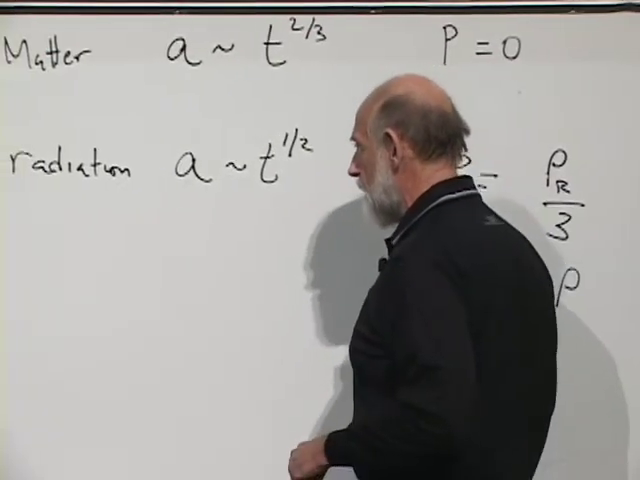
\includegraphics[width=0.74\textwidth]{lecture_04_figure_04.png}
\caption{物質與輻射：\(a\sim t^{2/3}\)、\(P=0\)；以及 \(a\sim t^{1/2}\)、\(P=\rho/3\)。}
\end{figure}

黑板上的摘要是
\begin{align}
\text{matter:}\qquad & a(t)\sim t^{2/3}, \qquad P=0,\\
\text{radiation:}\qquad & a(t)\sim t^{1/2}, \qquad P=\frac{\rho}{3}.
\end{align}

\begin{classroomqa}
\lecturetimestamp{00:54:27}
\audiencequestion{在膨脹的宇宙中，粒子不是實際上正在彼此遠離嗎？}
\lecturerresponse{是的，但壓力的論證是針對無窮小的共動盒子進行。在這個局部尺度上，熱力學推理仍然成立。}
\end{classroomqa}

\section{狀態方程}

我們假設壓力與能量密度成正比，
\begin{equation}
P=w\rho .
\end{equation}
黑板上用 \(\omega\) 表示同一個參數。兩種基本情況分別是
\begin{equation}
w=0 \quad \text{for cold matter},
\qquad
w=\frac{1}{3} \quad \text{for radiation}.
\end{equation}

也可能有介於 \(0\) 和 \(1/3\) 之間的值，代表既非完全冷態、也非完全相對論性的物質。這裡提到的例子是溫暖暗物質。

\begin{figure}
\centering
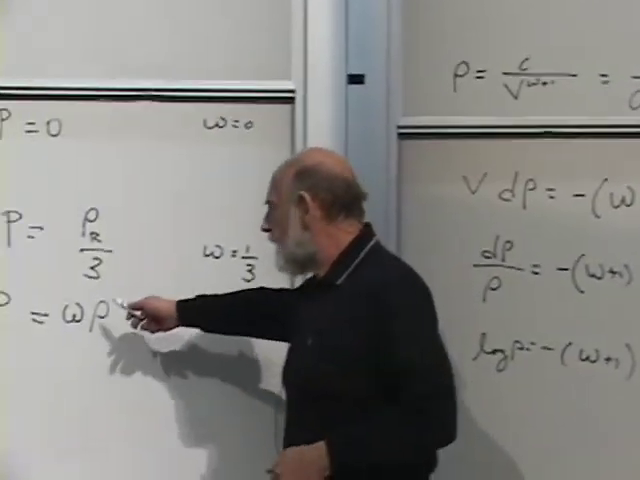
\includegraphics[width=0.74\textwidth]{lecture_04_figure_05.png}
\caption{狀態方程 \(P=\omega\rho\) 與密度標度的推導。}
\end{figure}

接下來要問的是，\(w\) 是否決定 \(\rho\) 對 \(a\) 的依賴關係。答案可由熱力學恆等式推得。

取一個體積為 \(V\) 的盒子。如果盒中物質施加壓力 \(P\)，那麼盒子膨脹 \(dV\) 時，對盒壁所做的功為
\begin{equation}
dE=-P\,dV.
\end{equation}
現在將能量寫成
\begin{equation}
E=\rho V.
\end{equation}
其微分為
\begin{equation}
dE=\rho\,dV+V\,d\rho .
\end{equation}
令兩個表示式相等，得到
\begin{equation}
\rho\,dV+V\,d\rho=-P\,dV,
\end{equation}
也就是
\begin{equation}
V\,d\rho=-(\rho+P)\,dV.
\end{equation}
利用 \(P=w\rho\)，可得
\begin{equation}
V\,d\rho=-(1+w)\rho\,dV.
\end{equation}
兩邊除以 \(\rho V\)：
\begin{equation}
\frac{d\rho}{\rho}=-(1+w)\frac{dV}{V}.
\end{equation}
積分後，
\begin{equation}
\rho \propto V^{-(1+w)}.
\end{equation}
對共動的宇宙學盒子而言，
\begin{equation}
V\propto a^3,
\end{equation}
因此
\begin{equation}
\rho \propto a^{-3(1+w)}.
\end{equation}

立刻就能得到前面討論的情況：
\begin{align}
w=0 &\Longrightarrow \rho \propto a^{-3},\\
w=\frac{1}{3} &\Longrightarrow \rho \propto a^{-4}.
\end{align}

這就是 \(w\) 重要的原因。知道 \(\rho(a)\) 之後，就能將它代回弗里德曼方程。接著設 \(a\sim t^\alpha\) 為冪律形式，便可求出該狀態方程下宇宙的膨脹方式。

\section{真空能與負壓力}

有一種特殊情況有所不同：
\begin{equation}
w=-1.
\end{equation}
於是
\begin{equation}
1+w=0,
\end{equation}
指數項便為零，因此
\begin{equation}
\rho=\rho_0=\text{constant}.
\end{equation}
相應的壓力為
\begin{equation}
P=-\rho .
\end{equation}

負壓力本身並不神秘。正壓力會向外推盒壁；負壓力則向內拉，也就是張力。拉緊的橡皮筋就是日常生活中的例子：它儲存正能量，卻會把兩端拉在一起。

把常數密度 \(\rho_0\) 代入弗里德曼方程：
\begin{equation}
\left(\frac{\dot a}{a}\right)^2=\frac{8\pi G}{3}\rho_0.
\end{equation}
右側只是常數，因此
\begin{equation}
\frac{\dot a}{a}=\sqrt{\frac{8\pi G}{3}\rho_0}.
\end{equation}
這是哈伯參數確實為常數的特殊情況。方程可以寫成
\begin{equation}
\dot a=\sqrt{\frac{8\pi G}{3}\rho_0}\,a,
\end{equation}
其解為
\begin{equation}
a(t)\propto \exp\!\left(\sqrt{\frac{8\pi G}{3}\rho_0}\,t\right).
\end{equation}

這就是指數膨脹。相關的時間尺度是 \(e\) 倍增時間，而不是加倍時間；這裡採用的粗略估計指出，它的量級約等於宇宙年齡。除歷史上採用的數值慣例外，真空能與宇宙學常數指的是同一種物理成分。

\begin{classroomqa}
\lecturetimestamp{01:27:16}
\audiencequestion{如果真空能驅動指數膨脹，最後所有東西不都會被撕裂嗎？}
\lecturerresponse{不一定。束縛系統可以抵抗膨脹。星系、太陽系或原子不一定會被撕裂；但夠大且稀疏的結構會隨宇宙膨脹，最後彼此分離。}
\end{classroomqa}

\begin{classroomqa}
\lecturetimestamp{01:31:43}
\audiencequestion{對弗里德曼方程開平方時，負號有什麼值得注意之處嗎？}
\lecturerresponse{有。開平方後會得到兩個分支：一個是膨脹解，另一個是時間反演後的收縮解。方程本身容許這兩種解。}
\end{classroomqa}

\section{三個時代與觀測到的膨脹歷史}

三種組分都存在，而且密度隨尺度因子的變化方式各不相同：
\begin{equation}
\begin{aligned}
\rho_{\text{radiation}}&\propto a^{-4},\\
\rho_{\text{matter}}&\propto a^{-3},\\
\rho_0&=\text{constant}.
\end{aligned}
\end{equation}
這立刻導出三個時代。

當 \(a\) 極小時，輻射佔主導。之後由物質佔主導。當 \(a\) 足夠大時，真空能佔主導。相應的膨脹定律為
\begin{equation}
a(t)\sim t^{1/2},
\qquad
a(t)\sim t^{2/3},
\qquad
a(t)\sim e^{Ht}.
\end{equation}

這裡引用的粗略時間如下：大約經過 \(10^4\) 年後，輻射主導轉為物質主導。大約經過 \(10^5\) 年後，宇宙才變得透明。物質主導轉為加速膨脹則晚得多，發生在數十億年後；依此處採用的數量級估算，約在宇宙歷史的中點。

我們如何推斷這段歷史？我們看不到未來，但看得到過去。觀測距離越遠，就越是在看更早的時刻。觀測遙遠星系、測量其運動與距離的關係，再重建哈伯參數隨回溯時間的變化，就能重建尺度因子的時間演變。輻射主導時代太早，無法透過一般星系天文觀測直接看見；但從重建曲線中，可以看見物質主導時代以及轉入真空能主導的過程。

\section{遙遠未來的最後散射}

未來的微波天空與星系越過視界而消失，是兩回事。我們在較晚時刻看到的輻射來自更遠處的物質，因此我們看到的是更深、更冷的宇宙，而不是看著同一批原子單純地退行遠去。

\begin{classroomqa}
\lecturetimestamp{01:48:07}
\audiencequestion{如果最後散射面逐漸隱沒在視界中，這和星系移到視界之外是同一回事嗎？}
\lecturerresponse{不是。較晚時刻看到的輻射，並非來自我們現在看到的同一批原子，而是來自更遠處的原子。這就像我們越看越深入宇宙，同時看到的輻射也越來越冷。}
\end{classroomqa}

\section{曲率、大擠壓圖像與晚期視界}

到目前為止，曲率項都省略了。把它加回來，得到
\begin{equation}
\left(\frac{\dot a}{a}\right)^2
=
\frac{8\pi G}{3}\rho
-
\frac{K}{a^2}.
\end{equation}
這一項的數值看起來很小，但在概念上很重要。用較早期的牛頓力學語言來說，它區分總能量為正、為零和為負的情況；用相對論的語言來說，它區分不同的空間幾何。

過去人們還沒有認真看待真空能時，常設想一個由物質主導、膨脹最終會反轉的宇宙。這就是舊有的大擠壓圖像：宇宙從大爆炸開始膨脹，之後再度收縮。這套數學仍然成立，但看來已不適用於我們的宇宙。

\begin{classroomqa}
\lecturetimestamp{01:53:51}
\audiencequestion{這種真空能和量子真空能有關嗎？}
\lecturerresponse{有關，至少一般相信兩者有關。}
\end{classroomqa}

目前宇宙的組成大致為
\begin{equation}
\frac{\rho_0}{\rho_{\text{total}}}\sim 0.7,
\qquad
\frac{\rho_{\text{matter}}}{\rho_{\text{total}}}\sim 0.3.
\end{equation}
在物質組分中，發光物質約佔總量的 \(0.05\)，暗物質約佔 \(0.25\)。目前輻射所佔的比例可以忽略。暗物質和發光物質的密度以相同方式隨尺度因子變化，因此即使物質、輻射和真空能的相對含量隨時代改變，兩者的比例仍固定。

在真空能主導的極限下，
\begin{equation}
H=\sqrt{\frac{8\pi G}{3}\rho_0}.
\end{equation}
於是哈伯定律變為
\begin{equation}
v=Hd.
\end{equation}
視界定義為 \(v=1\)，所以其距離為
\begin{equation}
d_H=\frac{1}{H}
=
\frac{1}{\sqrt{8\pi G\rho_0/3}}.
\end{equation}
這裡給出的粗略數值約為 \(10\) 至 \(12\) 十億光年。

重要的是晚期的行為。膨脹一旦進入指數形式，視界距離就會固定。星系仍會越過視界，並因紅移愈來愈大而消失。微波背景也會逐漸紅移到不可見。在遙遠未來，只有附近受引力束縛的結構仍可觀測，宇宙看起來會像一座孤島。

\section{從最後散射面測量幾何}

最後，可以透過最後散射面來檢驗幾何。假設我們已知到該表面的距離，也能在那裡辨認出一個物理大小已知得夠準確的團塊。接著就能把它的大小和距離與觀測到的角大小作比較。

在平坦空間中，角度符合歐幾里得幾何。在正曲率空間中，物體看起來會較大；在負曲率空間中則會較小。這就像一般測量：對已知距離、已知大小的物體測量角度，再與歐幾里得幾何的預測比較。

\begin{classroomqa}
\lecturetimestamp{02:08:09}
\audiencequestion{有什麼遠方物體的大小是我們已知的？}
\lecturerresponse{微波背景中最大的團塊。我們認為，從它們演化所需的時間以及聲速，可以推知其大小。}
\end{classroomqa}

這裡考慮的是微波背景中最大的團塊。觀測到的角大小與歐幾里得幾何的預測相符，差異在百分之幾以內。根據這項結果，空間看來是平坦的。

\section{測得的 \(w\) 與最後一個問題}

現在可以看出 \(w\) 在觀測上的重要性。如果天文學家報告說 \(w\) 非常接近 \(-1\)，他們的意思是真空能組分幾乎是常數。這正是這裡要指出的重點。

這並不表示廣義相對論迫使 \(w\) 恰好等於 \(-1\)。這裡談的是經驗結果。講座簡短提到，原則上不能排除更激進的可能性；但有充分理由相信，真空能近乎為常數的情況確實成立。

\begin{classroomqa}
\lecturetimestamp{02:11:04}
\audiencequestion{在計算物質和輻射的密度時，我們是否先假設能量保持不變，再調整尺度因子來求出公式？如果前兩種情況都是如此，那麼真空能的情況又如何？在那種情況下，密度保持不變。}
\lecturerresponse{不，我沒有假設能量保持不變。我們用的是能量變化量 \(-P\,dV\)。對於一個假想的共動盒子，它隨著宇宙膨脹而移動，膨脹時會對盒壁做功，這就解釋了能量的變化。真空能的情況引出了另一個問題；最後要補充的是，在宇宙學中談能量守恆意義不大，因為宇宙的總能量為零。}
\end{classroomqa}
\chapter{球面、雙曲空間與\(k\)的意義}

我們先做一點簡單的數學。任意維度的球面都是特殊的幾何：它們具有均勻性，也就是曲率為常數。先看正曲率，再看均勻負曲率，接著再說明它們與愛因斯坦方程的關係。

球形宇宙是指\emph{空間}是球形的，而不是時空。另一種可能性是具有均勻負曲率。把這兩種情形並列比較，才能看清廣義相對論的作用。

\section{球面與均勻幾何}

一維球面就是圓。描述它最簡單的方式，是將它嵌入二維輔助空間，並寫成
\begin{equation}
x^2+y^2=R^2.
\end{equation}
單位一維球面則是
\begin{equation}
x^2+y^2=1.
\end{equation}

二維球面也用同樣的方式描述，只是現在要用三個輔助座標：
\begin{equation}
x^2+y^2+z^2=R^2,
\end{equation}
單位球面的情形為
\begin{equation}
x^2+y^2+z^2=1.
\end{equation}

這些座標只是輔助工具。我們關心的幾何並不是周圍的\(x,y,z\)空間，而是球面本身。生活在一維球面上的生物生活在圓上，無法接觸圓的內部或外部。二維球面也是如此。球面內部的填充部分和球面外部，都只是輔助圖像的一部分。

同樣的構造也能得到三維球面。再引入一個座標，例如\(w\)，並寫成
\begin{equation}
x^2+y^2+z^2+w^2=R^2,
\end{equation}
單位球面的情形為
\begin{equation}
x^2+y^2+z^2+w^2=1.
\end{equation}
三維球面較難想像，因為輔助工具現在是四維的，但數學並沒有困難多少。

標準記號是用\(\Omega_n\)表示\(n\)維球面。因此，\(\Omega_1\)是一維球面，\(\Omega_2\)是二維球面，\(\Omega_3\)是三維球面。

\section{球面上的度量}

更實用的描述方式是內在描述，也就是用定義在球面本身的座標來描述球面。

描述單位一維球面只需要一個座標\(\phi\)，其範圍為\(0\leq \phi \leq 2\pi\)。它的度量為
\begin{equation}
ds^2=d\phi^2.
\end{equation}
也可以寫成
\begin{equation}
d\Omega_1^2=d\phi^2.
\end{equation}

單位二維球面可以視為一系列的一維球面。角度\(\phi\)仍沿著每個圓繞行，而另一個角度\(\theta\)則從球面的一端延伸到另一端。這個角度的範圍是\(0\)到\(\pi\)。沿\(\theta\)方向的位移對度量的貢獻是\(d\theta^2\)。而沿\(\phi\)方向繞行時，所在圓的半徑為\(\sin\theta\)。因此
\begin{equation}
d\Omega_2^2=d\theta^2+\sin^2\theta\,d\phi^2
\end{equation}
或寫成
\begin{equation}
d\Omega_2^2=d\theta^2+\sin^2\theta\,d\Omega_1^2.
\end{equation}

三維球面也以同樣的方式構造，現在可視為一系列的二維球面。引入另一個座標\(\alpha\)，則
\begin{equation}
d\Omega_3^2=d\alpha^2+\sin^2\alpha\,d\Omega_2^2.
\end{equation}
展開後為
\begin{equation}
d\Omega_3^2=d\alpha^2+\sin^2\alpha\left(d\theta^2+\sin^2\theta\,d\phi^2\right).
\end{equation}
此處，\(\alpha\)從一端的零尺寸延伸到另一端，因此\(0\leq \alpha \leq \pi\)。\editorialnote{00：17：24時，音訊聽起來短暫像是說了``零到二{\proseunicodefont π}''；但依照整個構造，以及明確出現的\(\sin^2\alpha\)因子，新座標必須從這一系列低維球面由零尺寸開始的一端，延伸至另一端。}

一般的遞迴形式為
\begin{equation}
d\Omega_n^2=d\alpha^2+\sin^2\alpha\,d\Omega_{n-1}^2.
\end{equation}

採用這種觀點後，就可以不再理會嵌入圖像。一維球面由一個座標描述，二維球面由兩個座標描述，三維球面由三個座標描述，以此類推。這種幾何本身就是完整的。

這種幾何之所以特殊，是因為它具有齊性。若將\(\sin^2\theta\)換成另一個在兩端仍為零的函數，就能改變度量，得到變形後的閉曲面，例如橢球面。但這樣的曲面就不再均勻。球面具有齊性，因為每一點都與其他各點相同。

若要描述半徑為\(A\)而非單位半徑的球面，只要將單位球面的度量乘上\(A^2\)：
\begin{equation}
ds^2=A^2\,d\Omega_3^2.
\end{equation}
必須取平方，因為度量衡量的是距離的平方。

順帶一提，零維球面可以由構造向前推一步得到：
\begin{equation}
x^2=1,
\end{equation}
其解為兩個點\(x=\pm 1\)。因此，單位零維球面就是兩個點。

\section{球形 FRW 宇宙}

現在關心的不只是空間，而是時空。相關的圖像是一個半徑隨時間變化的三維球面。

有一點必須始終謹記：時間是不同的。不要把膨脹中的宇宙想成高維球面，並把時間當作另一個嵌入座標。

有了這個認識，時空間隔為
\begin{equation}
d\tau^2=dt^2-a(t)^2\,d\Omega_3^2.
\end{equation}
這是空間為球形的宇宙所對應的 FRW 度量。相較於靜態球面，唯一的新成分是半徑變成了時間的函數\(a(t)\)。

將我們選在某個極點上，會讓座標較方便。那個位置並沒有任何特殊之處，這只是座標約定。如此一來，\(\alpha\)可以視為單位球面上從我們所在位置向外的徑向座標。它不是以公里為單位的徑向距離，而是單位球面上的無因次角度量，只是在幾何中扮演徑向距離的角色。

除星系、恆星等局部團塊之外，這就是空間為球形的 FRW 宇宙的完整幾何。它的空間曲率為正，符號約定寫作
\begin{equation}
k=+1.
\end{equation}
這本身並不是``加一''，而是表示空間曲率為正。

\section{從球面向外觀看}

從球面上的某一點向外看，這樣的球面會呈現什麼樣子？這就要用到球極投影。

取一個在南極與無限平面相切的二維球面。在球面上選一點，從北極穿過該點畫一條直線，並延長至與平面相交。如此一來，球面上的每一點都會映射到平面上的一點。南極會映射到平面的原點。北極則是例外：從不同方向接近北極時，它的像會沿著不同方向延伸至無窮遠。因此，我們將北極視為無窮遠點。

若在球面不同位置放上大小相同的``大陸''，它們在平面上的像會在接近北極時逐漸變大。因此，若觀察者位於南極，遠方物體所張的角會比在平坦空間中更大。在正曲率空間中，已知大小的物體相對於歐幾里得幾何看起來會過大。

這就是基本的觀測概念：根據距離、物體大小與角大小之間的關係推斷曲率。星系本身並不是測量極遠距離的理想標準尺，但推理方式正是如此。

\begin{classroomqa}
\lecturetimestamp{00:45:54}
\audiencequestion{除了角大小之外，還需要知道距離嗎？}
\lecturerresponse{需要。光知道角度還不夠，也必須知道距離。}
\end{classroomqa}

\begin{classroomqa}
\lecturetimestamp{00:46:18}
\audiencequestion{球面上的圓投影後仍會是圓嗎？}
\lecturerresponse{會。圓會投影成圓，這是球極投影的一項特殊性質。}
\end{classroomqa}

\begin{classroomqa}
\lecturetimestamp{00:47:02}
\audiencequestion{大陸經過投影後會維持原有形狀嗎？}
\lecturerresponse{這裡有兩個不同的說法。一個是圓會投影成圓；另一個較弱的說法是，足夠小的形狀會保留其局部形狀，因為角度不變。這種映射是保角的：它保留角度，但不保留相對大小。}
\end{classroomqa}

\section{均勻負曲率}

均勻負曲率的情形，會從度量開始介紹。

球面的負曲率類比是雙曲空間。依照前面相同的遞迴構造，將\(\sin\alpha\)換成\(\sinh\alpha\)，便可得到它的度量：
\begin{equation}
d\mathcal H_n^2=d\alpha^2+\sinh^2\alpha\,d\Omega_{n-1}^2.
\end{equation}
低維的角向部分仍是單位球面度量\(d\Omega_{n-1}^2\)。

\begin{classroomqa}
\lecturetimestamp{00:55:51}
\audiencequestion{度量中的低維微分項仍然是球面的那一項嗎？}
\lecturerresponse{是。低維部分就是一般的單位球面度量。改變的是它前面的\(\sinh^2\alpha\)因子。}
\end{classroomqa}

雙曲正弦為
\begin{equation}
\sinh\alpha=\frac{e^\alpha-e^{-\alpha}}{2}.
\end{equation}
負號很重要；講座中一位學生隨即指出並更正了這個符號。

座標範圍也有一項關鍵差異。在球面上，新座標從一端延伸至另一端，並在\(\pi\)處結束。在這裡，
\begin{equation}
0\leq \alpha<\infty.
\end{equation}
一般正弦先增大，然後又回到零。雙曲正弦在\(\alpha=0\)附近起初也有相似的行為，但接著會呈指數增長。

這表示，沿著這種幾何向外移動時，周圍的低維球面會愈來愈大。在這種幾何中，半徑增加時，天空不會先變大再縮小，而是持續擴大。

在三個空間維度中，相應的 FRW 形式為
\begin{equation}
d\tau^2=dt^2-a(t)^2\,d\mathcal H_3^2,
\end{equation}
其曲率符號標記為
\begin{equation}
k=-1.
\end{equation}

\section{圓盤圖像及其意義}

負曲率可以透過埃舍爾的圓盤圖像直觀呈現，尤其是\emph{《極限圓 IV》}。它和球極投影的類比很有用，但兩者的表現恰好相反。

球面的投影看起來無限延伸，但實際幾何是有限的；負曲率的圓盤圖像看起來有限，但實際幾何是無限的。大小相同的``大陸''或``星系''愈接近邊界，看起來就愈小，但在幾何上，它們的大小完全相同。若以經過多少個等大區塊來計量距離，邊界就位於無窮遠處。

因此，在負曲率空間中，已知大小的物體相對於平坦空間看起來太小，所張的角也太小。

這種幾何仍然具有均勻性。雖然圖像中外側區域看起來很小，但若將觀察者移到其他位置，他看到的內在幾何仍會相同。

\begin{classroomqa}
\lecturetimestamp{01:06:42}
\audiencequestion{如果觀察者位於其中任一個圓內，也會看到類似的圖樣嗎？}
\lecturerresponse{會，完全相同。空間具有均勻性。}
\end{classroomqa}

\begin{classroomqa}
\lecturetimestamp{01:07:03}
\audiencequestion{在球面情形中，遠處物體看起來太大；在這裡則看起來太小嗎？}
\lecturerresponse{是。在正曲率空間中，已知大小的物體相對於平坦空間所張的角太大；在負曲率空間中，所張的角太小。}
\end{classroomqa}

\begin{classroomqa}
\lecturetimestamp{01:08:09}
\audiencequestion{這種類似球極投影的投影，是否能讓天文學家從觀測結果重建幾何？}
\lecturerresponse{是。天文學家實際上就像測量師，測量天空中的三角形。就目前要說明的幾何概念而言，可以先不考慮時間變化，專注於角度和距離。}
\end{classroomqa}

還有一個有用的局部圖像：可以把一小塊負曲率空間畫成普通三維空間中的馬鞍面。但只能這樣表示局部區域；整個雙曲平面無法完整嵌入普通三維歐幾里得空間，成為一個形狀良好的曲面。

\section{平坦情形}

介於正曲率與負曲率情形之間的是平坦空間。可以把它看成一種極限，不過只要將它視為一般的平坦歐幾里得空間即可。

它的 FRW 形式為
\begin{equation}
d\tau^2=dt^2-a(t)^2\left(dx^2+dy^2+dz^2\right),
\end{equation}
其中
\begin{equation}
k=0.
\end{equation}

這就是三種均勻 FRW 幾何：
\begin{align}
k=+1 &: \text{positive spatial curvature},\\
k=0 &: \text{flat space},\\
k=-1 &: \text{negative spatial curvature}.
\end{align}

\begin{classroomqa}
\lecturetimestamp{01:15:07}
\audiencequestion{若將幾何投影到平面上並追蹤一個訊號，投影中光速會隨位置改變嗎？}
\lecturerresponse{會，在投影圖像中會如此。在球面投影中，愈往外看，光似乎移動得愈快；在負曲率圓盤中，愈接近邊緣，光似乎移動得愈慢。這種變化只出現在圖像中，並不屬於底層物理。}
\end{classroomqa}

\begin{classroomqa}
\lecturetimestamp{01:17:05}
\audiencequestion{人們真的曾用這種方式觀察遠方物體來判定空間是否平坦嗎？}
\lecturerresponse{有，但實際使用的是角度資訊。判定空間是否平坦，並不是靠測量光在投影圖像中看起來移動得多快。}
\end{classroomqa}

\section{回到宇宙學方程}

休息之後，接下來要說明先前研究過的宇宙學方程與愛因斯坦方程之間的關係。此時黑板上仍留有平坦空間度量的一部分。

\begin{figure}[htbp]
\centering
\includegraphics[width=0.72\textwidth]{lecture_05_figure_02.png}
\caption{平坦 FRW 度量片段。}
\lectureframe{01:18:18}
\end{figure}

首先簡短回顧牛頓力學。把我們放在中心，觀察一個依照哈勃定律遠離我們的星系。根據牛頓的球對稱分布定理，只有該星系距離所對應半徑的球體內部質量，會對它所受的力有所貢獻。於是有三種可能：星系的運動速度高於逃逸速度、低於逃逸速度，或恰好等於逃逸速度。

接著回顧，對一般非相對論物質而言，密度與質量除以\(a^3\)成正比；對輻射而言，密度則與\(1/a^4\)成正比；而真空能的密度不會隨球體大小改變。

先前的牛頓力學處理中，宇宙學方程包含一個密度項；若不是恰好處於逃逸速度的情形，還會多出一個正比於\(1/a^2\)的常數項。先前的討論大多將此項設為零。從經驗上看，此項很小，但在概念上沒有理由將它省略。

\section{愛因斯坦方程與\(00\)分量}

接下來看愛因斯坦場方程。左側是由時空曲率構成的幾何，右側則是作為引力場源頭的能量動量張量。按照講座採用的歸一化，方程寫成
\begin{equation}
R^{\mu\nu}-\frac{1}{2}g^{\mu\nu}R=4\pi G\,T^{\mu\nu}.
\end{equation}
\editorialnote{黑板上可見的方程中，因子\(\tfrac12\)無法辨認，但在01:33:36附近，講者口頭更正時補上了這個因子。此處的方程採用更正後的形式，並保留講座中的\(4\pi G\)歸一化。}

此處不需要用到十個獨立分量中的每一個。到目前為止，我們已經作了許多假設---包括均勻性、FRW 形式，以及只有一個隨時間變化的尺度因子---因此只剩下一個任意函數，也就是\(a(t)\)。自然的選擇是時間—時間分量，因為\(T^{00}\)就是能量密度\(\rho\)。

\begin{figure}[htbp]
\centering
\includegraphics[width=0.62\textwidth]{lecture_05_figure_05.png}
\caption{愛因斯坦場方程及其\(00\)分量。}
\lectureframe{01:30:54}
\end{figure}

因此，焦點是
\begin{equation}
R^{00}-\frac{1}{2}g^{00}R=4\pi G\,\rho.
\end{equation}

右側是能量密度，左側是幾何。

\begin{classroomqa}
\lecturetimestamp{01:39:09}
\audiencequestion{能量動量張量的其他分量呢？}
\lecturerresponse{一般而言，它們不為零。空間—空間分量可以表示壓力。在物質主導的情形中，壓力為零；在輻射主導的情形中，壓力是能量密度的三分之一；對真空能，則寫作\(P=w\rho\)，其中\(w=-1\)。}
\end{classroomqa}

\begin{classroomqa}
\lecturetimestamp{01:40:24}
\audiencequestion{所以，如果只有物質，\(T^{\mu\nu}\)的其他分量會消失嗎？}
\lecturerresponse{對無壓物質而言，會，壓力分量為零。}
\end{classroomqa}

\section{愛因斯坦計算的結果}

講者沒有在黑板上完整推導曲率。重點在於將 FRW 度量代入愛因斯坦張量後會出現什麼結果。

其中一類項只來自尺度因子隨時間變化這件事。即使空間是平坦的，隨時間變化的尺度因子仍會產生時空曲率。這項貢獻正比於
\begin{equation}
\left(\frac{\dot a}{a}\right)^2.
\end{equation}

第二類項來自空間本身的曲率。即使尺度因子固定不隨時間變化，彎曲空間仍會對時空曲率有所貢獻。對於簡單且均勻彎曲的幾何，曲率與曲率半徑的平方成反比，因此會產生一個正比於
\begin{equation}
\frac{k}{a^2},
\end{equation}
的項；球面情形為正號，雙曲情形為負號，平坦空間則為零。

\begin{classroomqa}
\lecturetimestamp{01:36:53}
\audiencequestion{是否還應該有像曲率半徑那樣的因子？}
\lecturerresponse{那已經包含在\(1/a^2\)因子裡了。對這些簡單而均勻彎曲的幾何而言，曲率就是曲率半徑平方的倒數。}
\end{classroomqa}

推導過程中即席處理了係數，也部分參照先前的牛頓力學結果進行核對。最後得到\footnote{這個弗里德曼方程形式，整合了講者口頭討論並自行修正的係數，以及在01:32:35--01:36:53附近與先前牛頓力學結果所作的比較。}
\begin{equation}
\left(\frac{\dot a}{a}\right)^2+\frac{k}{a^2}=\frac{8\pi G}{3}\rho,
\end{equation}
或等價地寫成
\begin{equation}
\left(\frac{\dot a}{a}\right)^2=\frac{8\pi G}{3}\rho-\frac{k}{a^2}.
\end{equation}

這個形式將三種 FRW 幾何與先前討論的宇宙動力學連結起來。

\begin{classroomqa}
\lecturetimestamp{01:37:52}
\audiencequestion{如果重新定義\(a\)，\(k\)可以取任意值嗎？}
\lecturerresponse{在平坦情形下，\(a\)沒有唯一自然的尺度，所以可以重新縮放，但\(k\)仍為零。在球面與負曲率情形下，則存在自然的曲率尺度。若令\(a(t)\)等於這個自然的曲率半徑，\(k\)就只是\(+1\)或\(-1\)。}
\end{classroomqa}

\begin{classroomqa}
\lecturetimestamp{01:41:00}
\audiencequestion{在最後的方程中，\(k\)等於\(+1\)、\(-1\)還是\(0\)？}
\lecturerresponse{是。球面情形為\(+1\)，雙曲情形為\(-1\)，平坦空間則為\(0\)。}
\end{classroomqa}

牛頓力學的處理沒有誤導我們；它得到了相同的基本方程。廣義相對論補上的是詮釋。從牛頓力學的觀點來看，額外的常數用來區分運動速度高於逃逸速度、低於逃逸速度，以及恰好等於逃逸速度的臨界情形。從愛因斯坦的觀點來看，同一個符號則代表空間本身的幾何。

\begin{classroomqa}
\lecturetimestamp{01:42:46}
\audiencequestion{還沒有納入宇宙學常數時，這套關係是如何成立的？}
\lecturerresponse{在引入宇宙學常數之前，逃逸速度的運動情形與空間幾何之間有緊密的對應關係。若\(k=+1\)，空間曲率為正，運動速度低於逃逸速度，因此宇宙可以先膨脹再收縮。若\(k=-1\)，空間曲率為負，運動速度高於逃逸速度，因此宇宙會持續膨脹。若\(k=0\)，則是臨界的刀鋒情形。}
\end{classroomqa}

因此，同一個符號\(k\)可以從兩種角度解讀：一是運動的動力學分類，二是空間曲率的符號。

\chapter{最後散射與重子生成}

\section{向外看，就是向過去看}

在不同距離上，我們看到的是宇宙在不同時期的樣貌。在近處，回溯時間並不太重要。一年前或一百年前的宇宙，和現在的宇宙並沒有太大差異。但到了足夠遠的地方，我們看到的就是較年輕的宇宙。宇宙越年輕，密度越高；密度越高，溫度也越高。

在某個足夠遠的距離上，宇宙的溫度大約和太陽表面相當。它在我們看來並非如此，因為光子在來到這裡的途中已經發生紅移。紅移因子約為一千，表示觀測到的溫度也降低了相同的倍數：
\[
T_{\mathrm{obs}} \sim \frac{T_{\mathrm{emit}}}{1+z},
\qquad
1+z \sim 10^3.
\]\footnote{這是對00:02:20--00:02:39口頭紅移論證的簡要編輯轉錄。}

那就是宇宙變得不透明的地方。宇宙的主要成分是氫，另有少量氦。溫度高於幾千度時，氫會電離。因此，在那個表面之外，存在的不是中性原子，而是離子：主要是自由運動的質子和電子。那裡的光子能量也更高，基本上是 X 射線。如果偶然形成原子，它很快就會再次被碰撞或光子電離。

電離氣體是導電體，而導電體無法讓輻射順利穿透。電荷會對電場作出反應，來回振盪，並重新發射輻射。因此，在那個距離之外，宇宙對我們而言是不透明的。最後散射面就像太陽的可見表面：它不是一道物質構成的牆，而是介質從不透明突然轉為透明的地方。

那裡的粒子絕大多數是光子，數量約為其他粒子的\(10^8\)倍。今天也是如此，儘管現在光子的能量很低，因此在當前的能量密度中並不重要。一旦溫度降到氫的電離溫度以下，宇宙就變得透明，我們也就能看穿它。

我們的直接觀測到此為止。接下來的問題是，已知的原子、核子與粒子物理，還能讓我們追溯到多早以前。

\section{追溯到更早以前}

就在最後散射面內側，除了光子之外，主要的粒子是質子和電子，還有一些氦核和少量氘核。幾乎沒有反質子，也幾乎沒有正電子。但再往更早以前，溫度終究會高到足以讓兩個光子碰撞，產生一個電子和一個正電子：
\[
\gamma + \gamma \leftrightarrow e^- + e^+.
\]

基本的閾值條件是，光子至少必須提供這一對粒子的靜止能量：
\[
E \ge 2m_e c^2.
\]
低於這個閾值，普通的光無法做到這一點。高於閾值，就能產生電子--正電子對，逆反應也可能發生。在這種溫度下，一鍋熱物質會包含各種粒子反應，就像普通物質中會發生化學反應一樣。

溫度剛高於閾值時，光子仍多於電子和正電子。電子的靜止質量需要很高的能量才能產生。但溫度遠高於閾值時，電子的靜止能量相較於動能便不再重要，粒子密度也會變得相近。此時，電子、正電子和光子的密度大致相同，彼此猛烈碰撞。

\begin{figure}[ht]
\centering
\includegraphics[width=0.62\textwidth]{lecture_06_figure_02.png}
\caption{比較電子與質子質量尺度的對產生閾值示意圖。}
\lectureframe{00:18:47}
\end{figure}

接下來的問題是質子會如何變化。質子已經存在，而且當時的密度很高，但熱能還不足以大量產生質子--反質子對。原因很簡單：
\[
m_p \approx 2000\,m_e,
\qquad
E \ge 2m_p c^2
\]
這是高得多的閾值。\editorialnote{圖中較低處的質量標記不如上方的\(2m_e c^2\)清晰，但口頭比較明確指的是電子與質子的閾值。}

這已經比恆星內部熱得多；在恆星內部，反粒子的豐度並不顯著。

但即使如此，也只是一種暫時的描述。溫度高到足以自由產生質子和反質子時，也高到足以把質子撞散成夸克。因此，真正熾熱的粒子湯，更適合描述為由電子、正電子、夸克、反夸克、光子、中微子、膠子及其他粒子種類組成。黑板上的一個簡單示意反應是
\[
e^- + e^+ \to \gamma \to q + \bar q.
\]

\begin{classroomqa}
\lecturetimestamp{00:20:05}
\audiencequestion{是介子，還是前夸克？}
\lecturerresponse{介子由夸克組成。溫度一旦高到足以打碎質子，也會打碎介子。}
\end{classroomqa}

到目前為止，推理的方向是回溯時間。現在把方向倒過來，看看這鍋熾熱而對稱的粒子湯冷卻時會發生什麼。

\section{電中性與對稱的熱宇宙}

在足夠高的溫度下，宇宙中粒子和反粒子的密度都極高。電子與正電子成對出現，夸克與反夸克也成對出現；自然的圖像是，每種粒子和它的反粒子數量幾乎相等。

電中性這件事需要稍加說明。今天的宇宙是電中性的。一個有用的助記方式是：想像一個閉合且有限的宇宙，例如三維球面，而不是我們實際的宇宙。先用二維球面作為模型來思考。電場線只能在電荷處起始或終止。正電荷發出力線，負電荷吸收力線。在閉合球面上，這些力線不能直接逃到無窮遠，而會在對側重新匯聚。因此，作為助記，閉合且有限的宇宙不能帶有淨電荷。我們的宇宙是否真的閉合，並不是重點。重點是，大尺度上的正、負電荷似乎抵消得極為精確。

電中性\emph{並不}表示質子數和反質子數相同。它表示總正電荷等於總負電荷。質子、正電子以及所有其他帶正電的粒子種類，其電荷總和，必須與電子及所有其他帶負電的粒子種類的電荷總和相平衡。

在已知物理學仍可信的範圍內，或許還能再往前推一點，宇宙曾經熱到足以讓粒子和反粒子大量存在。任何能想到的加速器實驗，在早期宇宙的某個階段都有對應的過程。近乎對稱的起始狀態是很自然的猜想：電子與正電子數目相等，夸克與反夸克數目相等；此外，若以質子和反質子代表重子和反重子，則
\[
N_p = N_{\bar p}.
\]

這個猜想很有吸引力，因為物理定律對粒子和反粒子幾乎對稱。正電子的行為和電子非常相似，雖非完全相同，但相差極微。問題就在於這種近乎對稱。

\section{把電影向前播放}

假設宇宙從一個熾熱狀態開始，粒子和反粒子的豐度相等或幾乎相等，接著逐漸冷卻。

只要溫度夠高，質子和反質子就能由高能碰撞產生，也能湮滅成光子。但溫度終究會降到質子產生閾值以下。此時，質子--反質子對仍能湮滅成光子；然而，宇宙膨脹一段時間後，這些光子損失了足夠的能量，就無法再轉變成質子--反質子對。這就成了單行道。之後，電子和正電子也會發生同樣的事；當時的溫度遠低於質子閾值，但仍遠高於恆星內部的溫度。

在這個過程中，宇宙膨脹的速度遠低於微觀反應速率，因此大部分時間都接近熱平衡。這裡所說的絕熱膨脹，指的就是這種情況。更精確地說，熵的變化非常小。對於熾熱的粒子湯，熵大致等於粒子數，兩者相差的因子約為一。因此，湮滅掉的質子、反質子、電子和正電子，大致由光子取代。

如果質子和反質子的數目完全相等，它們就會全部湮滅。電子和正電子也會如此，最後只剩下光子。但如果質子數哪怕只比反質子數多一點，成對的粒子會湮滅，未配對的多餘部分則會留下來。舉例來說，如果有一百個質子和五十個反質子，五十個反質子會各自找到一個質子，與之湮滅，最後留下五十個質子。電中性也要求電子相對於正電子留下同樣形式的多餘數量。

由今天的光子數，可以推知早期的不對稱程度。今天的光子數約為質子數或電子數的\(10^9\)到\(10^{10}\)倍：
\[
\frac{N_\gamma}{N_p} \sim 10^9\text{--}10^{10}.
\]
所以，在早期熾熱的粒子湯中，大約每一對質子--反質子就多出一個質子。原子之所以至今仍然存在，全靠這微小的不平衡。

\begin{classroomqa}
\lecturetimestamp{00:42:25}
\audiencequestion{為什麼不從統計角度來看這個多出的部分，把它視為冷卻過程中以極小機率產生的結果？}
\lecturerresponse{若要從初始對稱的狀態中多出一個質子，就必須在不產生反質子的情況下產生質子；同時還必須產生與它相伴的負電荷，例如電子。已知的標準模型並沒有這種低能過程。在那些經過檢驗的能量範圍內，重子數守恆，因此一般的冷卻過程不會產生淨多出的重子。}
\end{classroomqa}

所以電荷並不是障礙。示意例子如下：
\[
\gamma + \gamma \to p + e^-.
\]\footnote{這是對00:44:16--00:46:35口頭例子的編輯轉錄，目的是單獨說明：電荷可以守恆，而重子數可以不守恆。}
整體而言，這會是電中性的。但它違反了另一條經驗規則。在已檢驗的標準模型中，產生質子時不能不產生反質子。就目前的討論而言，相關的守恆量是重子數：
\[
B=(N_p+N_n)-(N_{\bar p}+N_{\bar n}).
\]\footnote{這個簡要公式將00:45:18--00:45:40處的口頭定義形式化。}
在已知能量範圍內，重子數守恆，因此這種不對稱不可能在冷卻過程後期、也就是物理學已充分經過檢驗的階段中產生。

\section{重子生成}

這個問題稱為重子生成。假設宇宙起初的重子和反重子數目確實相等。物理定律必須允許什麼，才能讓這個對稱狀態偏向一方，形成觀測到的微小多餘量？

黑板上將問題歸結為兩個符號表示式：
\[
N_p=N_{\bar p},
\qquad
N_p-N_{\bar p},
\]
接著列出一系列條件，說明如何從第一個狀態轉變為第二個狀態。

\begin{figure}[ht]
\centering
\includegraphics[width=0.72\textwidth]{lecture_06_figure_04.png}
\caption{由初始對稱狀態產生重子不對稱的條件。}
\lectureframe{01:22:26}
\end{figure}

\editorialnote{這個畫面中的編號列表只有部分文字清晰可辨。以下三項是根據隨附的口頭說明整理而成。}

第一個條件是重子數不守恆。如果重子數是精確的守恆量，那麼起初淨重子數為零的宇宙，就會一直維持淨重子數為零。

第二個條件是粒子和反粒子之間必須有所偏向。只有重子數不守恆還不夠。如果自然界允許產生質子的過程，以及與之對應、產生反質子的過程，兩者發生的機率相同，平均的不平衡仍然是零。兩者的反應速率必須不同。

一般的統計漲落也遠遠不夠。如果粒子總數約為\(10^{90}\)，其中包括光子，那麼大小約為\(\sqrt{N}\)的漲落只能產生大約\(10^{45}\)，遠不足以解釋宇宙中約有\(10^{80}\)個質子。

第三個條件是，宇宙必須曾在某個時期充分偏離平衡。這裡的論證用到 CPT 定理。如果一團熱氣體永遠處於平衡，倒著播放它的演化，和正著播放看起來會一樣。在這種情況下，結合電荷共軛、宇稱和時間反演的精確對稱性，會有效地恢復粒子與反粒子之間的對稱。要讓真正的偏向留下來並固定下來，實際的歷史在微觀時間尺度上，正向與反向演進時必須有所不同。在宇宙早期，膨脹速度曾足夠快，因此能做到這一點。

因此，三個條件是：
\begin{enumerate}
\item 重子數不守恆；
\item 粒子與反粒子之間的對稱性遭到破壞，更精確地說，是 CP 對稱性破壞；
\item 曾有一個偏離熱平衡的階段。
\end{enumerate}

\begin{classroomqa}
\lecturetimestamp{01:09:08}
\audiencequestion{對照 CPT 定理來看，條件2確實指 CP 破壞，而條件3確實指時間方向的問題嗎？}
\lecturerresponse{是的。條件2確實應該表述為 CP 破壞。條件3指的是實際歷史曾偏離平衡；它不是一條獨立的守恆定律，也不等同於重子數不守恆。}
\end{classroomqa}

有了這三個條件，即使宇宙起初的質子和反質子數目相等，也可能產生偏向其中一方的不平衡。尚未確定的是，自然界是否真的存在重子數不守恆；如果存在，具體機制又是什麼。

\section{已知與未知}

尚未解決的部分是重子數不守恆。我們從未在自然界中直接觀測到會改變
\[
(N_p+N_n)-(N_{\bar p}+N_{\bar n}).
\]
的反應。這可能只是表示，相關反應所需的溫度遠高於實驗室直接測試過的任何溫度；也可能是因為它們在低能下發生的機率極低。但目前這仍是個問號。

這就是質子衰變在這場討論中如此重要的原因。如果重子數不是精確守恆量，原則上質子就應該不穩定。但質子極其穩定。此處引用的壽命下限約為
\[
\tau_p \gtrsim 10^{34}\ \text{years}.
\]
這個結果來自大型實驗：實驗使用大量裝設光偵測器的水，並將設備深埋在地下。它不能證明重子數不會不守恆，只表示任何此類效應在低能下都必須受到極強的抑制。

討論中也提到一項已知物理。在\(100\)到\(250\,\mathrm{GeV}\)附近，弱相互作用會變得更像電磁相互作用。這對詳細模型可能很重要，但並不是當前論證中的關鍵轉折。

暗物質不會大幅改變基本的論述。在多數理論中，暗物質與普通物質的作用非常微弱；就這個問題而言，它基本上只是旁觀者。

\begin{classroomqa}
\lecturetimestamp{01:24:49}
\audiencequestion{引力如何影響這一切？}
\lecturerresponse{主要有兩方面。第一，若沒有宇宙膨脹，就不會出現偏離平衡的階段。第二，黑洞蒸發有力地暗示，重子數不可能永遠是精確的守恆量。除此之外，粒子間一般的引力作用太弱，在這裡影響不大。}
\end{classroomqa}

接著有一個關於電荷的問題：同樣的黑洞論證是否也會威脅電荷守恆？答案是否定的。帶電黑洞具有向外延伸的電通量線，而這些線保留著電荷的資訊。這種黑洞不會完全蒸發，而會逐漸接近極端黑洞的殘餘態。因此，黑洞論證威脅的是重子數守恆，不是電荷守恆。

另一個問題是，極度緻密的早期夸克湯是否應該直接視為黑洞。答案是否定的。關鍵不在於一團靜止的緻密物質；當時的宇宙正在膨脹。黑洞的例子是用來思考重子數可能的命運，並不是說早期宇宙實際上是個受困區域。

\begin{classroomqa}
\lecturetimestamp{01:31:14}
\audiencequestion{人們知道如何修改標準模型，納入這類反應嗎？}
\lecturerresponse{問題恰好相反。要加入過多的重子數不守恆效應很容易，結果會使質子衰變得太快。真正的難題是，既要讓早期宇宙中所需的過程得以發生，又要讓質子維持目前這樣的穩定性。}
\end{classroomqa}

\section{熵與後期的中子問題}

現在回頭整理一下。在絕熱膨脹的宇宙中，熵近似守恆。對於由基本粒子組成的熱粒子湯，熵大致等於粒子數，兩者相差的因子約為一。因此，這個討論不需要假設宇宙後期憑空產生大量光子。湮滅主要是把粒子湯的成分重新分配成輻射。

這個問題的舊版本把因果關係說反了。當時問的不是為什麼相較於光子只有這麼少的質子存留下來，而是反過來問：為什麼相較於質子有這麼多光子？但更精確的問題不是宇宙為什麼在後期產生這麼多熵，而是粒子與反粒子的初始不對稱為什麼這麼小：大約每一對質子--反質子中，只多出一個質子。

自由中子確實會衰變，但這個過程\emph{並不}違反重子數守恆：
\[
n \to p + e^- + \bar\nu.
\]
中子的重子數和質子相同。

自由中子衰變時，可用的衰變能量很小，因為中子的質量只比末態的質量稍大。這也是它的衰變速度以基本粒子的標準來看相當緩慢的原因之一。中子若束縛在原子核中，結合能可能完全抵銷這一點可用能量，於是束縛中子便能保持穩定。

\begin{classroomqa}
\lecturetimestamp{01:43:03}
\audiencequestion{中子只是從宇宙中消失，還是也會有中子產生？}
\lecturerresponse{首先，自由中子會因衰變而減少。但這不是全部情況。中子確實也會透過某些過程產生，例如恆星中的核反應和中子星的形成。因此，中子的總數並非只會一路減少。}
\end{classroomqa}
\chapter{真空能量、暴脹與原初漲落}

\section{真空能量與德西特空間}

在平坦空間中，弗里德曼方程為
\begin{equation}
\left(\frac{\dot A}{A}\right)^2=\frac{8\pi G}{3}\rho.
\end{equation}
對物質而言，\(\rho\)按\(A^{-3}\)的比例下降；對輻射而言，\(\rho\)按\(A^{-4}\)的比例下降。真空能量則不會稀釋：
\begin{equation}
\rho=\rho_0=\text{constant}.
\end{equation}
如果宇宙中只有這種真空能量，方程右側便是常數。將這個常數寫成\(H^2\)，
\begin{equation}
H^2=\frac{8\pi G}{3}\rho_0,
\qquad
H=\sqrt{\frac{8\pi G}{3}\rho_0}.
\end{equation}
哈勃常數便是真正的常數：
\begin{equation}
\frac{\dot A}{A}=H.
\end{equation}
因此
\begin{equation}
\dot A=HA,
\end{equation}
解呈指數形式：
\begin{equation}
A(t)=C e^{Ht}.
\end{equation}
彼此遙遠且不受束縛的星系之間，距離會按指數增長。這就是德西特空間。

在這些座標下，時空幾何為
\begin{equation}
d\tau^2=dt^2-e^{2Ht}\left(dx^2+dy^2+dz^2\right).
\end{equation}
此處的真空能量為正。在平坦空間中，它必須為正，因為弗里德曼方程左側非負。負的真空能量只有在納入曲率項時才可能出現，而這裡討論的並非那種情況。

愛因斯坦引入宇宙常數，原本是為了另一個目的：平衡普通物質，讓宇宙維持靜態。

\section{當今加速膨脹的宇宙}

德西特空間也是當今宇宙晚期演化的趨勢。較早時，標度因子遵循物質主導時的關係
\begin{equation}
A(t)\propto t^{2/3}.
\end{equation}
幾十億年前，曲線開始向上彎，增長速度也逐漸加快。由於仍有其他形式的能量存在，膨脹還不是完美的指數形式，但趨勢正朝此方向發展。

這裡所說的加速是指
\begin{equation}
\ddot A>0.
\end{equation}
這是宇宙晚期膨脹的一項觀測特徵。

現在來看視界。哈勃定律表示
\begin{equation}
v=HD.
\end{equation}
在退行速度等於光速的距離處，
\begin{equation}
D=\frac{c}{H}.
\end{equation}
等價地，也可以改寫為\(HD=c\)。\editorialnote{這是將口頭說明的關係式\(D=c/H\)以代數方式重新表述。圖~\ref{fig:lecture07-horizon}右側黑板最上方那一行只有部分可辨。}

\begin{figure}[ht]
\centering
\includegraphics[width=0.62\textwidth]{lecture_07_figure_02.png}
\caption{德西特膨脹中的宇宙視界關係\(D=c/H\)。}
\label{fig:lecture07-horizon}
\lectureframe{00:30:37}
\end{figure}

這個距離約為一百億至一百五十億光年；若將宇宙年齡用\(c\)換算成距離，數值也相近。

\begin{classroomqa}
\lecturetimestamp{00:14:10}
\audiencequestion{視界尺度與宇宙年齡幾乎相等，難道不正是切線恰好通過原點時會出現的情況嗎？}
\lecturerresponse{若是\(A(t)\propto t\)，那就完全成立。但一般而言並非如此。在德西特空間中，\(H\)維持不變，宇宙年齡卻持續增加，因此目前兩者幾乎相等並非數學上的恆等關係。}
\end{classroomqa}

\section{真空能量的意義}

這裡以普通量子力學的語言描述真空能量。諧振子的能量概略可寫成
\begin{equation}
E\sim p^2+x^2.
\end{equation}
在古典力學中，基態就是平衡點：
\begin{equation}
x=0,\qquad p=0,\qquad E=0.
\end{equation}
量子力學不允許\(x\)和\(p\)同時精確為零。不確定性原理使系統必然有漲落，因此基態能量為正。諧振子的基態能量為
\begin{equation}
E_0=\frac{1}{2}\hbar\omega.
\end{equation}

接著將同樣的想法應用於場。宇宙中充滿諧振子：電磁場的振盪，以及其他每一種場的振盪。每種場都有零點能。電磁場的能量密度概略可寫成
\begin{equation}
u_{\mathrm{EM}}\sim E^2+B^2.
\end{equation}
即使沒有真實光子，仍存在無法消除的零點振盪。這是真空能量的一種解釋。此處只需要知道，這種能量確實存在，而且不會隨宇宙膨脹而稀釋。

\begin{classroomqa}
\lecturetimestamp{00:16:15}
\audiencequestion{真空能量究竟是什麼？如果移除物質和輻射，為什麼仍有能量留下？}
\lecturerresponse{因為真空是量子場的基態，而量子基態的能量不一定為零。諧振子的基態能量為正，而場可以視為諧振子的集合。因此，即使沒有真實粒子，仍有零點能存在。}
\end{classroomqa}

這不是三度背景輻射。微波背景是普通輻射，其能量密度會下降，因為光子數密度降低，而且每個光子都會紅移。真空能量則是移除真實光子後仍留下的零點能。

\section{\(H^{-1}\)的意義}

現在回到倒數哈勃常數與宇宙年齡之間的關係。如果
\begin{equation}
A(t)\propto t,
\end{equation}
那麼
\begin{equation}
H=\frac{\dot A}{A}=\frac{1}{t}.
\end{equation}
更一般地，若
\begin{equation}
A(t)\propto t^p,
\end{equation}
那麼
\begin{equation}
H=\frac{p}{t}.
\end{equation}
對物質主導的情況\(p=2/3\)而言，
\begin{equation}
H=\frac{2}{3t}.
\end{equation}
因此，在冪律宇宙模型中，\(H^{-1}\)與宇宙年齡同量級，但不會恰好等於宇宙年齡。

德西特空間則不同。在那裡
\begin{equation}
A(t)=C e^{\gamma t},
\end{equation}
因此
\begin{equation}
H=\frac{\dot A}{A}=\gamma,
\end{equation}
是個真正的常數。此處的\(H^{-1}\)不是宇宙年齡，而是指數增長的時間常數：標度因子增為原來\(e\)倍所需的時間。口頭講解中一再說``加倍''，隨即又更正；精確的說法是增為\(e\)倍。如今，這個時間常數約為一百億年。

\begin{classroomqa}
\lecturetimestamp{00:23:46}
\audiencequestion{能否再說明一次宇宙年齡和倒數哈勃常數之間的關係？}
\lecturerresponse{冪律膨脹下可得\(H=p/t\)，所以\(H^{-1}\)與宇宙年齡相差一個約為一的因子。但在德西特空間中，\(H\)維持不變，宇宙年齡卻持續增加，因此\(H^{-1}\)代表的是指數膨脹的時間常數，而非宇宙年齡。}
\end{classroomqa}

\section{能量與宇宙視界}

如果真空能量密度在宇宙膨脹時維持不變，自然會讓人想知道真空總能量是否正在增加。這裡的回答有所限度。在廣義相對論中，能量的帳目還包含引力的部分，因此總能量的概念比初等力學中更為微妙。實際上，此處要把握的是與視界相關的要點。

在精確的德西特空間中，宇宙視界的大小固定：
\begin{equation}
D=\frac{c}{H}
=\frac{c}{\sqrt{8\pi G\rho_0/3}}.
\end{equation}
因此，視界內的體積也固定。當中的真空能量為
\begin{equation}
E_{\mathrm{hor}}=\frac{4\pi}{3}D^3\rho_0.
\end{equation}
\editorialnote{這是對00：31：06--00：32：23口頭計算的簡要整理：取視界尺度，計算球體體積，再乘以\(\rho_0\)。}
由於\(D\)和\(\rho_0\)都是常數，這個量不隨時間改變。對特定觀測者而言，在精確的德西特空間中，他所能觀測到的宇宙範圍內，真空能量維持不變。

物體也可能穿越宇宙視界，情況大致如同穿越黑洞視界。一旦到了視界之外，它們便與我們失去因果聯繫。

\begin{classroomqa}
\lecturetimestamp{00:29:27}
\audiencequestion{如果真空能量密度在宇宙膨脹時維持不變，多出來的能量從哪裡來？}
\lecturerresponse{講座以廣義相對論的觀點作答，而不是把宇宙想成牛頓力學中的盒子。在精確的德西特空間中，視界大小固定，因此永遠可被觀測到的區域內，真空能量也維持不變。}
\end{classroomqa}

\section{為何引入暴脹}

接著把同樣的德西特機制推演到遙遠的過去，只是當時的時間常數短得多，約為
\begin{equation}
H^{-1}\sim 10^{-32}\,\mathrm{s}.
\end{equation}
這就是暴脹的構想：在任何可直接觀測的時期之前，宇宙曾經歷一段指數膨脹。

基本動機在於宇宙的平坦與均勻。空間切片看來非常平坦；在大尺度上，宇宙也非常均勻。更引人注目的是，最後散射面本身就已經相當均勻，因此這種均勻化不可能只發生在後來可見的宇宙歷史中。

放癟的氣球表面皺縮不平；把它吹得夠大，任何可見的局部區域都會顯得平滑。葡萄乾或西梅也能說明相同的道理：皺縮的物體經過極大的拉伸後，在任何可見區域看來都會平滑。暴脹理論認為，宇宙正是如此變得平滑。

這也回答了此處所談的視界問題。最後散射面上相距遙遠的區域都能被我們觀測到，但在後來可見的宇宙歷史中，光沒有足夠時間從一個區域傳到另一個區域。因此，這些區域的密度和溫度幾乎一致，暗示在更早的時期，它們曾屬於同一個較小區域，之後才被大幅拉伸。

暴脹有利也有弊。它消除了宇宙對初始條件的敏感性；同樣地，也抹去了關於宇宙如何開始的許多資訊。

平坦性問題在此以更明確的形式再度出現。觀測上，曲率參數\(k\)看來為零，精確度約達百分之一或更高。在可見區域內，空間幾何看來是歐幾里得的。暴脹的解釋是，曲率半徑遠大於我們能觀測到的區域。

\begin{classroomqa}
\lecturetimestamp{00:40:05}
\audiencequestion{我們是否假設暴脹之前宇宙處於平衡狀態？}
\lecturerresponse{不是。暴脹的想法幾乎正好相反。此前不論有什麼結構，都會被大幅拉伸，使可見區域不再保留那些早期細節的資訊。}
\end{classroomqa}

\section{標量場及其位能}

為了解釋早期宇宙的有效真空能為何可能遠高於現在，可以引入一個標量場。電場和磁場都是向量，與它們不同，標量場沒有方向；它在每個位置只有一個值：
\begin{equation}
\phi=\phi(x,y,z,t).
\end{equation}
這是個假設性的場，並未對應自然界中任何已知的場，其量子也未對應任何已知粒子。

此處關鍵的能量部分是位能：
\begin{equation}
V(\phi).
\end{equation}
所謂``位能''，是指與場本身的值相關的能量，而不是與場的時間導數相關的能量。\(\phi\)取不同值時，能量也可能不同。

\begin{figure}[ht]
\centering
\includegraphics[width=0.68\textwidth]{lecture_07_figure_03.png}
\caption{定性的標量位能\(V(\phi)\)，顯示不同的場值對應不同的位能。}
\label{fig:lecture07-generic-potential}
\lectureframe{00:47:08}
\end{figure}

\begin{classroomqa}
\lecturetimestamp{00:46:34}
\audiencequestion{\(V(\phi)\)圖中的橫軸代表什麼？}
\lecturerresponse{橫軸代表場值\(\phi\)，縱軸代表位能\(V\)。}
\end{classroomqa}

如果場在空間和時間上維持定值，或在關注區域內近似定值，那麼\(V(\phi)\)的作用就與真空能量完全相同：不會稀釋。因此，先前的德西特公式只要將\(\rho_0\)替換為\(V(\phi)\)，便可沿用。特別是，
\begin{equation}
H=\sqrt{\frac{8\pi G}{3}V(\phi)}.
\end{equation}

如果\(\phi\)隨位置而變，不同區域的暴脹時間常數就會不同。但只要拉伸幅度夠大，任何可見區域都會變得近乎均勻。

\begin{classroomqa}
\lecturetimestamp{01:05:11}
\audiencequestion{這裡的\(\phi\)是否相當於時間參數？}
\lecturerresponse{在這段討論中，有限度地說是如此：場沿位能曲線演化時，它是時間的單調函數。}
\end{classroomqa}

\section{平臺、懸崖與再加熱}

這個圖景所需的位能曲線有一段非常平坦、但並非完全平坦的區域；接著到達懸崖邊緣，急遽下降，沒有完全降到零，之後又上升。

\begin{figure}[ht]
\centering
\includegraphics[width=0.68\textwidth]{lecture_07_figure_04.png}
\caption{具有高平臺、陡降區與較低極小值的暴脹位能。}
\label{fig:lecture07-inflationary-potential}
\lectureframe{01:02:30}
\end{figure}

這種形狀是高度人為設計的，但之所以提出這種模型，是因為宇宙學圖景似乎需要類似的結構。

場從平臺高處開始演化。由於斜率很小，而且膨脹所造成的有效黏滯很大，\(\phi\)變化得非常緩慢。石頭在蜂蜜中緩慢下沉，比物體在桌面上滑動更接近此處要表達的圖景。宇宙膨脹得越快，這種黏滯效應就越大。

\begin{classroomqa}
\lecturetimestamp{00:59:07}
\audiencequestion{是什麼在推動\(\phi\)演化？}
\lecturerresponse{推動它的是位能曲線的斜率。斜率很小，而宇宙學上的黏滯效應很大，所以場值變化緩慢，不會快速演化。}
\end{classroomqa}

當\(\phi\)沿著平臺緩慢演化時，\(V(\phi)\)幾乎不變。因此，宇宙的暴脹近似於真空能量維持不變時的情況。這個階段的時間常數約為
\begin{equation}
H^{-1}\sim 10^{-32}\,\mathrm{s}.
\end{equation}
口頭粗略估計，平臺高度以普朗克單位表示約為\(10^{-14}\)。\editorialnote{這是01:14:38--01:14:47口頭提出的``最佳猜測''，並非講座中推導出的數值。}

暴脹持續了多久？目前無從得知，因為平臺的寬度和坡度都不清楚。已知的是，宇宙至少膨脹了約\(e\)的五十倍，而通常引用的數字是六十倍。\editorialnote{這是對01:14:05--01:19:27口頭所談指數膨脹次數的編輯性重述。}這些次數以指數膨脹單位計：每一次都使尺度增為\(e\)倍。

當場值演化到懸崖邊緣時，位能會迅速下降。場的位能先轉化為動能，再轉化為熱和粒子，宇宙因而變得熾熱。這裡所說的``再加熱''一詞略有誤導，因為暴脹期間，先前任何熱能都已被稀釋殆盡。

較低的極小值並不在零處。該處留下的小位能，正是與當今緩慢的指數膨脹相關的能量。

\begin{classroomqa}
\lecturetimestamp{01:19:48}
\audiencequestion{平臺能否完全平坦，再由擾動以某種方式把場推離邊緣？}
\lecturerresponse{不能。位能曲線不可能完全平坦，必須帶有一定斜度。若平坦得過頭，再加熱後的宇宙就會過於不均勻。}
\end{classroomqa}

``大爆炸''在此有兩個相近的含義：可以指再加熱事件本身，也可以指最早能直接觀測到的階段，也就是最後散射面。關鍵在於，實際觀測到的一切都遠低於暴脹平臺。

\begin{classroomqa}
\lecturetimestamp{01:45:42}
\audiencequestion{再加熱本身就是大爆炸嗎？}
\lecturerresponse{你若願意，可以這麼說。但當時宇宙仍然極為熾熱且不透明。最後散射面出現得晚得多，那時宇宙已冷卻到足以變得透明。}
\end{classroomqa}

\section{量子漲落與星系的種子}

暴脹使可見宇宙變得非常均勻，但並非完全均勻。若沒有量子漲落，場會變得完全平滑；但量子力學使場在不同位置仍有微小差異。

核心圖像以縱向表示一般空間，橫向表示場值\(\phi\)。如果場完全均勻，在給定時刻，空間中每一點的\(\phi\)都會相同，而且各處會同步朝懸崖邊緣演化。如此一來，每個區域都會在同一時刻越過懸崖。量子漲落打破了這種完全同步。

兩個圖像可以說明這一點：一個是在原本均勻的場中出現小凸起；另一個是一排手挽手走向懸崖的士兵。若他們完全排齊，就會一起跌落；若有人稍微領先，有人稍微落後，他們就會在不同時刻越過懸崖。

接下來是關鍵效應。較早越過懸崖的區域會較早再加熱。等較晚的區域越過懸崖時，較早越過的區域已經膨脹了一段時間，也稍微冷卻了。這種差異會造成再加熱後的能量密度變化。

\begin{classroomqa}
\lecturetimestamp{01:34:00}
\audiencequestion{較晚再加熱的區域，比較早再加熱的區域更熱還是更冷？}
\lecturerresponse{較早再加熱的區域已有時間膨脹並冷卻。因此，較晚再加熱的區域在越過懸崖時溫度較高，這種差異也會造成密度不均勻。}
\end{classroomqa}

觀測到的效應很小：
\begin{equation}
\frac{\delta\rho}{\rho}\sim 10^{-5},
\end{equation}
約為十萬分之一。這些是原初密度漲落，並非暗能量。此處並未單憑定性圖像推導出這個數值；而是用它來限制平臺的高度與平坦程度。

這些漲落也是必要的。沒有它們，就不會有星系。再加熱之後，引力會放大初始的漲落圖樣。過密區會從欠密區吸引物質，於是過密區變得更密，欠密區則更稀，最終形成後來的星系和恆星結構。

這不只是定性的說法。可以計算膨脹宇宙中場的量子漲落，追蹤它們經過再加熱後的演化，再將結果與從星系分布重建的漲落圖樣比較。兩者符合得相當好。

這段討論也帶出熵的問題。引力造成物質結團，看來有違直覺，但並不違反熱力學第二定律。引力在統計力學中很特別：它傾向於使物質結團，而結團會提高熵，不會降低熵。

\begin{classroomqa}
\lecturetimestamp{01:40:24}
\audiencequestion{既然\(\phi\)不是電磁場，微波背景在這整個過程中如何反映這些漲落？}
\lecturerresponse{原初密度漲落的圖樣會留在最後散射面上。再加熱將場能轉化為普通粒子和光子，之後微波背景便帶有這些原初漲落留下的印記。}
\end{classroomqa}

\section{聲學振盪與下一步}

最後，討論簡短轉向聲學振盪。它們發生在後來引力造成結構成團之前。原初漲落會演化成聲學振盪，並在天空留下物理尺度已知的斑塊。

這很重要，因為在已知距離處，已知的物理尺度便能充當量尺。測量它在最後散射面上所張的角度後，就能運用幾何判斷空間是平坦、正曲率還是負曲率。詳細內容留待後續討論。

\begin{classroomqa}
\lecturetimestamp{01:47:19}
\audiencequestion{聲學振盪呢？}
\lecturerresponse{它們能在天空中充當量尺。已知的物理尺度，加上在最後散射面上觀測到的角尺度，讓我們得以測量空間幾何。詳細內容留待下一講再談。}
\end{classroomqa}
\chapter{暴脹、結構與初始條件的消失}

\section{{\proseunicodefont Ω}與平坦性的證據}

一位學生問到大\(\Omega\)，討論因此回到弗里德曼–羅伯森–沃克方程。就現在這個遠離輻射主導時期的宇宙而言，膨脹定律寫成真空能項與物質項；輻射項則因為已經非常小而略去：
\begin{equation}
H^2=\left(\frac{\dot a}{a}\right)^2=\frac{8\pi G}{3}\left(\rho_0+\rho_m\right)-\frac{k}{a^2}.
\end{equation}
真空項不會稀釋，物質項則會：
\begin{equation}
\rho_m=\frac{M}{a^3}.
\end{equation}
\(\Omega\)表示膨脹方程中各種組分所占的比例。

將方程兩邊除以\(H^2\)，各項經過歸一化後的總和便為一。採用經整理的記號，
\begin{equation}
\begin{aligned}
\Omega_0&=\frac{8\pi G\rho_0}{3H^2},\\
\Omega_m&=\frac{8\pi G\rho_m}{3H^2},\\
\Omega_k&=-\frac{k}{a^2H^2},
\end{aligned}
\end{equation}
因此
\begin{equation}
\Omega_0+\Omega_m+\Omega_k=1.
\end{equation}
\editorialnote{這一段的音訊與黑板內容都不太清楚，講者也在幾個名稱之間切換，指稱真空貢獻。此處將方程除以\(H^2\)後，整理了論證所用的記號。}
若空間是平坦的，\(k=0\)，因此
\begin{equation}
\Omega_0+\Omega_m=1.
\end{equation}
物質項與真空項之和若大於一，曲率為正；若小於一，曲率為負。

觀測上的推論很直接：測量普通物質與暗物質，測量哈勃膨脹，並在極大尺度上以幾何方法測量曲率。也要留意，宇宙正在加速。判斷真空項的符號，不能只看\(H\)本身，而要看\(\dot a/a\)趨近常數的趨勢；這表示尺度因子會趨近指數膨脹的形式，
\begin{equation}
a(t)\propto e^{Ht}.
\end{equation}
這些測量彼此交叉檢驗，顯示宇宙非常接近平坦，偏差只有百分之幾。

\begin{classroomqa}
\lecturetimestamp{00:10:50}
\audiencequestion{物質項包括暗物質嗎？}
\lecturerresponse{是。就目前的討論而言，物質項包括暗物質。也可以把輻射加進去，不過如今輻射所占的比例非常小，可以忽略。}
\end{classroomqa}

\begin{classroomqa}
\lecturetimestamp{00:11:11}
\audiencequestion{除了哈勃常數之外，還有其他方法可以衡量暗能量嗎？}
\lecturerresponse{重點不在\(H\)本身的數值，而在於膨脹如何趨近指數定律。再結合物質的測量結果，以及以幾何方法測得的平坦性，就能推論出真空項。}
\end{classroomqa}

\section{從平坦性到結構}

宇宙為什麼如此平坦？一種解釋是暴脹。平坦意味著宇宙在數十億、甚至數百億光年的尺度上非常大、非常平滑，也非常均勻。指數膨脹可以把一個區域拉伸到呈現這種樣貌。

不過，好事也可能做過頭。完全平滑的宇宙會一直保持完全平滑。引力無法從精確的對稱性中產生成團結構。既然現在存在結構，這些結構必定是從早期的微小不均勻性開始形成。將現在的宇宙往回追溯，到了透明時期，不均勻性的大小約為\(10^5\)分之一：
\begin{equation}
\frac{\delta\rho}{\rho}\sim 10^{-5}.
\end{equation}
當時的宇宙極其平滑，但並非完全平滑。

從那時起，引力便開始做出一般房間裡的空氣所受的普通力做不到的事。微小的過密區會把物質吸引過來，附近區域因此變得稀疏；於是欠密區愈加欠密，過密區愈加過密。引力會增強這種反差，而不是將它抹平。

自然會問，為什麼這種情況沒有更早發生。答案是壓力。早期的輻射壓很大。利用
\begin{equation}
p=w\rho,
\end{equation}
常見的情形是
\begin{equation}
w_{\rm rad}=\frac13,\qquad
w_m=0,\qquad
w_{\rm vac}=-1.
\end{equation}
正壓力會使介質趨於均勻，將擾動推開並使介質平滑。在大尺度上，物質可視為沒有壓力，因此不會提供這種支撐。有壓力時，引力受到抑制；壓力變得可以忽略時，引力便占上風。

暗物質對事件發生的先後順序至關重要。最先坍縮形成的是暗物質暈。接著，普通重子物質落入這些暈中；由於重子物質能夠耗散，會聚集到較靠近中心的地方。暗物質不會以同樣的方式耗散，因此仍分布在整個暈中。收縮大約在透明時期之前開始，時間上約早十倍；因此，微波背景並未直接呈現這一過程的起始。

插一句，交代後來的化學演化：幾乎所有比氦重的元素都是恆星演化的產物，而非早期宇宙學的產物。早期宇宙基本上只產生氫、氦，以及少量幾種輕原子核。

天空中觀測到的不是質量密度本身，而是微波背景的溫度各向異性。密度漲落會對它有所貢獻，速度漲落也會。過密區域往往看起來稍冷一些，因為光子離開較深的引力勢阱時會額外損失能量；此外，氣體運動造成的都卜勒頻移也會疊加其上。完整的數值分析相當複雜。較可靠、也較簡單的結論是：宇宙變得透明時，能量密度的變化約為\(10^5\)分之一。

\begin{classroomqa}
\lecturetimestamp{00:20:29}
\audiencequestion{為什麼引力沒有讓這些團塊更早增長？}
\lecturerresponse{因為早期宇宙由輻射主導，而輻射帶有足以使介質均勻化的正壓力。只有當輻射相較於物質變得不重要時，引力才開始主導團塊的增長。}
\end{classroomqa}

\begin{classroomqa}
\lecturetimestamp{00:24:35}
\audiencequestion{坍縮不需要耗散機制嗎？}
\lecturerresponse{普通重子物質要沉降到中心，確實需要耗散。但暗物質不必經過那種碰撞耗散，也能先形成暗物質暈。此外還有一種與膨脹本身有關的宇宙學阻尼，稍後會談到它的重要性。}
\end{classroomqa}

\begin{classroomqa}
\lecturetimestamp{00:30:34}
\audiencequestion{是否也有速度漲落，讓後來的星系能夠獲得角動量？}
\lecturerresponse{是。原初圖樣包含密度漲落與速度漲落。天空中觀測到的溫度圖樣，是由密度變化與氣體運動共同造成的。}
\end{classroomqa}

\section{暴脹子與平臺}

接下來介紹的機制涉及一個標量場\(\phi\)。它的能量密度由三部分組成：
\begin{equation}
\rho_\phi=\frac12\dot\phi^2+\frac12(\nabla\phi)^2+V(\phi).
\end{equation}
時間變化會有所貢獻，空間變化也會；標量場還可以帶有真正的勢能\(V(\phi)\)。這部分並不奇特，希格斯場就是熟悉的例子。關鍵在於勢能的形狀。

勢能在某個範圍內必須相當平坦，只有微微向下的斜坡；接著到了某個臨界值，勢能便陡然下降。它不會恰好降至零，而是降到非常小的值。以普朗克單位表示，當今的真空能量約為
\begin{equation}
10^{-123}.
\end{equation}
平臺上的能量比這大得多，但仍遠低於普朗克尺度。

\begin{figure}[t]
\centering
\includegraphics[width=0.78\textwidth]{lecture_08_figure_03.png}
\caption{定性示意暴脹子勢能：寬闊的平臺、陡降的斜坡，以及低處的極小值。}
\lectureframe{00:43:23}
\end{figure}

這張圖描述的不是空間中的位置，而是場的取值。說宇宙從平臺高處開始，只表示在一個極大的區域內，場值都位於那個高處。起初\(\phi\)在不同位置有些變化並不重要，因為暴脹會把這些變化大幅拉伸。膨脹得夠久之後，任何局部區域看起來都幾乎均勻。\editorialnote{黑板畫面中的座標軸標籤無法辨認，但口頭討論清楚指出，縱軸是勢能\(V(\phi)\)，橫軸是場值\(\phi\)。}

只要場停留在勢能寬闊且緩緩傾斜的部分，勢能的作用就像真空能。若\(\phi\)完全不變，它的作用便會和真空能完全相同。先不計省略的數值因子，講課中給出的關係就是
\begin{equation}
H\propto \sqrt{V(\phi)},
\end{equation}
由此得到近似指數膨脹定律
\begin{equation}
a(t)\propto e^{Ht}.
\end{equation}
如今能觀測到的幾乎一切，都發生在場越過斜坡邊緣之後。場從邊緣下降時，平臺上大量類真空能量便轉化為輻射、普通物質、暗物質，以及今天觀測到的微量殘餘真空能。

\begin{classroomqa}
\lecturetimestamp{00:44:07}
\audiencequestion{\(\phi\)是什麼場？這裡仍然使用愛因斯坦方程嗎？}
\lecturerresponse{是。\(\phi\)是時空上的場，而且仍然使用同一個弗里德曼方程。在這種情況下，只要場變化得夠慢，方程右側的能量密度就主要由\(V(\phi)\)提供。}
\end{classroomqa}

\begin{classroomqa}
\lecturetimestamp{00:47:04}
\audiencequestion{類真空的暴脹子能量如何轉化為物質和輻射？}
\lecturerresponse{場滾到谷底並開始振盪時，這些振盪就是場的量子。若這些量子不穩定，便可能衰變成光子、電子、正電子和其他熟悉的粒子。}
\end{classroomqa}

\section{慢滾與哈伯摩擦}

場越過斜坡邊緣後，為什麼不會一直來回振盪？為什麼不會來回擺動，甚至再度爬上去？這裡給出的答案是宇宙學阻尼機制。它並非真正的微觀摩擦，但在運動方程中的作用類似摩擦。

忽略空間梯度，將場視為均勻。如此一來，動能項與勢能項看起來就像一個具有\(T-V\)動力學的單一自由度；但因為它們是能量密度，必須乘上物理體積\(a^3\)。因此可得到如下形式的均勻有效拉格朗日量：
\begin{equation}
L_{\mathrm{hom}}=a^3(t)\left[\frac12\dot\phi^2-V(\phi)\right].
\end{equation}
\editorialnote{黑板最上方的一行被部分裁掉。這裡只在足以重現下方清楚寫出的運動方程的範圍內，重建這個均勻拉格朗日量。}

黑板上清楚寫出的方程是
\begin{equation}
\frac{d}{dt}\left(a^3\dot\phi\right)=-a^3\frac{\partial V}{\partial\phi}.
\end{equation}
展開時間導數後得到
\begin{equation}
a^3\ddot\phi+3a^2\dot a\,\dot\phi=-a^3\frac{\partial V}{\partial\phi},
\end{equation}
再除以\(a^3\)，便有
\begin{equation}
\ddot\phi+3H\dot\phi=-\frac{\partial V}{\partial\phi}.
\end{equation}
講者在口頭推導中明確更正了負號：力等於勢能對場的導數取負。

\begin{figure}[t]
\centering
\includegraphics[width=0.78\textwidth]{lecture_08_figure_05.png}
\caption{均勻暴脹子的運動方程，顯示哈伯摩擦項\(3H\dot\phi\)。}
\lectureframe{00:57:10}
\end{figure}

\(3H\dot\phi\)這一項稱為哈伯摩擦，完全來自對因子\(a^3\)微分。不過，就動力學而言，它看起來就像石塊落入水中時受到的阻力項。方程中有力項、加速度項，以及一個與速度成正比的項。場很快便達到終端速度，接著沿著平臺緩慢移動，這就是慢滾階段。斜坡平緩、場移動緩慢時，勢能變化也很慢，因此膨脹維持近似指數形式。

場在極小值附近振盪。這些振盪就是暴脹子量子。若這些量子不穩定，便會發生衰變，平臺上的能量也就藉此轉化為後期宇宙中的熱物質與輻射。

\begin{classroomqa}
\lecturetimestamp{00:50:48}
\audiencequestion{場為什麼不會一直振盪下去？阻尼從何而來？}
\lecturerresponse{膨脹本身會產生類似摩擦的項。均勻拉格朗日量中的因子\(a^3\)會產生\(3H\dot\phi\)項，其作用就像黏滯阻力。}
\end{classroomqa}

\section{量子漲落與越過視界}

現在看來似乎有個問題：若暴脹使宇宙變得極其平滑，為什麼沒有把星系所需的種子也抹掉？答案在於量子力學。留下來的漲落並非不完全平滑所殘留的痕跡，而是重新產生的。

先暫時不管膨脹。即使場幾乎完全均勻，量子力學仍不允許\(\phi\)與\(\dot\phi\)同時具有完全確定的值。基態仍然存在擾動，這和普通諧振子具有零點能是同一個原因。在日常情況下，這些漲落很難觀測，因為它們波長短、振盪快，觀測時會對它們取平均。

膨脹改變了情況。在共動座標中，場模態的座標波長大致不變，物理波長則隨尺度因子增長：
\begin{equation}
\lambda_{\rm phys}=a(t)\,\Delta x.
\end{equation}
暴脹期間，物理哈伯尺度近似固定，
\begin{equation}
d_H\sim H^{-1},
\end{equation}
因此相應的共動視界會以如下方式縮小：
\begin{equation}
d_{H,\mathrm{coord}}\sim \frac{1}{aH}.
\end{equation}

繩子的比喻有助於理解模態如何凍結。波會振盪，是因為繩子的每一小段都受到相鄰部分的牽引。但若波長大到和視界相當，相關的相鄰部分便超出因果接觸範圍，恢復力隨之消失。模態一旦長於視界，就會凍結。

這種情況不斷重演：長波長先凍結，短波長後凍結。即使某個模態起初的波長極短，最終也會被拉伸到越過視界。因此，暴脹並非只會抹去結構；它還會持續產生凍結的場變化。

即使暴脹持續很久，這個過程也不會停止。舊的凍結模態被拉伸到極大尺度，新的模態則不斷凍結。就宇宙學所關心的意義而言，累積而成的圖樣在統計上趨於穩定。近似尺度不變譜便由此而來：同一個越過視界的過程在接續的對數尺度上反覆發生，使相鄰波長帶的振幅大致相同。

場滾下平臺後，視界再度增長。先前位於暫時暴脹視界之外的模態，之後會重新進入視界。通常會說，這些模態在暴脹期間離開視界，之後又重新進入。此時它們已被拉伸至宏觀尺度，因此再次開始振盪時，呈現的是非常大的結構。

\begin{classroomqa}
\lecturetimestamp{01:12:02}
\audiencequestion{在時空圖上，視界看起來是什麼樣子？}
\lecturerresponse{指數膨脹期間，到視界的物理距離大致維持在\(c/H\)；但在共動座標圖上，由於座標尺度不斷被拉伸，這段固定的物理距離看起來會愈來愈短。換成共動距離來說，視界會按\(1/(aH)\)縮小。}
\end{classroomqa}

\begin{classroomqa}
\lecturetimestamp{01:15:59}
\audiencequestion{漲落被拉伸時，振幅會如何變化？會形成穩態嗎？}
\lecturerresponse{個別模態會在拉伸時稀釋，但新的模態不斷凍結。結果是形成統計上穩定、近似尺度不變的圖樣，而不是讓漲落完全消失。}
\end{classroomqa}

\section{從凍結的場變化到密度變化}

場在不同位置產生微小變化後，若不同區域越過斜坡邊緣的時間略有差異，這些變化便會轉化為密度差異。沿斜坡稍微更低處的區域會先到達邊緣。若它的真空能轉化為輻射，輻射便會隨膨脹而稀釋。相鄰區域若仍在平臺上，就仍由真空能主導，不會稀釋。等到第二個區域落下時，第一個區域已有一部分能量因紅移而流失。

這就是為什麼場滾動得愈慢，最後形成的密度反差愈大。若場沿著平臺移動得很慢，場值的微小差異便會使相鄰區域到達斜坡邊緣的時間差拉大。較早落下的區域有更多時間稀釋，等到較晚落下的區域才轉化其能量。斜坡愈平緩，終端速度愈小，最後的密度變化也愈大。平臺愈高，漲落通常也愈大。平臺寬度主要決定暴脹持續的時間。

漲落資料嚴格限制的，是能量高度與斜率的一種組合。若能量尺度夠高，也應會有可觀測的引力波貢獻。這裡給出的數值界限只是粗略估計。大致而言，若平臺上的能量密度遠高於約\(10^{-14}\)個普朗克單位，微波背景中就會出現過多的引力波訊號；若遠低於約\(10^{-16}\)個普朗克單位，實際上就很難觀測到這種訊號。\editorialnote{講者明確表示這些數值只是近似值，並說自己記不清確切數字。此處僅保留其數量級估計。}

單位依照自然單位制的慣例說明。質量為\(m\)的粒子，其康普頓波長為
\begin{equation}
\lambda_C=\frac{\hbar}{mc}.
\end{equation}
若\(c=\hbar=1\)，質量與長度的倒數便具有相同單位。能量密度是單位體積內的能量，因此其單位是質量的四次方：
\begin{equation}
[\rho]=(\mathrm{mass})^4.
\end{equation}

在單一位置觀察時，凍結模態的累積看起來像隨機漫步。空間中不同位置各自經歷不同的隨機漫步，正是這種差異將量子雜訊轉化為空間變化。

\begin{classroomqa}
\lecturetimestamp{01:33:04}
\audiencequestion{\(\phi\)會隨機漫步嗎？這是否使更早的起始狀態變得無關緊要？}
\lecturerresponse{在任一固定位置，相繼凍結的模態以隨機相位相加，因此\(\phi\)確實會隨機漫步。但這項成果本身也帶來了困難：暴脹不斷以後來的漲落取代早先的資訊，使暴脹之前的階段難以重建。}
\end{classroomqa}

\section{暴脹所隱藏的事物}

這個理論在一個特定意義上相當成功：它以同一個底層機制，連結起跨越巨大尺度範圍的漲落。但同一個機制也會沖淡此前的狀態。早期的不規則性被拉伸到難以察覺，之後產生的量子漲落則成為仍然重要的部分。因此，暴脹既引人注目，也令人困擾。它解釋了宇宙的平滑性與漲落譜，卻也抹去了大部分更早的歷史。

這讓人對起始狀態感到不安。問題不在於能量密度非常高，而在於平臺能量看起來既非自然落在普朗克尺度，也非自然地極小。以一般單位來看，它很高；但以普朗克單位來看，它仍然很小。它不像是基礎理論中一個顯而易見的起始位置。

在這個簡單圖像中，也沒有字面上的\(t=0\)。暴脹一旦持續太久，幾乎所有關於更早階段的資訊都會消失。若 e-fold 數只比所需的最小值略高，也許還能留下前一階段的某些痕跡；但一般而言，暴脹會抹去過去。

處理德西特空間時也有同樣的保留。純粹的指數定律適用於暴脹分支的晚期，但精確的德西特解更適合寫成
\begin{equation}
a(t)\propto \cosh(Ht).
\end{equation}
這個解會先收縮到最小尺度，然後再膨脹。收縮分支是否應在宇宙學中按字面理解，仍是個開放問題。

\begin{classroomqa}
\lecturetimestamp{01:37:31}
\audiencequestion{宇宙會不會沒有起點，而指數膨脹一直向過去延續？}
\lecturerresponse{在這個簡單圖像中不會。精確的德西特空間並非在所有時間都永遠指數膨脹；它更像\(\cosh(Ht)\)，包含收縮分支和膨脹分支。較早的那個分支是否應按字面理解，仍是個開放問題。}
\end{classroomqa}

\section{微調、曲率與人擇界限}

粗略來說，重要的參數包括平臺的高度、斜率與寬度\(\Delta\phi\)。斜率會決定終端速度，進而決定漲落大小，因此很重要；寬度則有助於決定暴脹持續多久。一種常見的看法是，基本的場位移不應遠大於普朗克質量，而能量密度不應超過普朗克單位下的一個量級。在這些粗略界限下，能產生足夠暴脹的參數並未遍及整個參數空間。此處引用的估計是，需要微調百分之幾，約為\(2\%\)，才能讓斜率足夠平緩，以產生約\(60\)至\(62\)個 e-fold。

\begin{classroomqa}
\lecturetimestamp{01:46:02}
\audiencequestion{能否用參數空間來理解暴脹？需要多大程度的微調？}
\lecturerresponse{可以。粗略來說，可以考慮平臺的高度、斜率與寬度。講課中提出的估計是，要有足夠的 e-fold 數，需要百分之幾程度的微調，約為\(2\%\)。}
\end{classroomqa}

接著，討論將這種程度不大的微調，與當前宇宙學常數的難題相比；後者的量級約為\(10^{-123}\)。話題轉向人擇問題，因為這兩個難題都可以改寫成：形成結構需要具備什麼條件？

在牛頓圖像中，正的宇宙學常數會造成一種與距離成正比的普遍斥力。若它大得多，不必等到今天把星系撕裂，就足以造成致命影響；只要大到能阻止原初\(10^{-5}\)漲落凝聚成星系即可。講者舉的例子是，若其數值約比觀測值高兩個數量級，就足以造成這種結果。這就是溫伯格論證的要點：宇宙學常數不必恰好為零，只須小到足以讓結構形成。

負曲率也會產生同方向的作用。用先前講課中的牛頓語言來說，\(k<0\)表示退行速度大於逃逸速度。向外推力若過強，也會使微小的原初過密區無法發展成星系。暴脹會稀釋這種曲率。引用的下界約為\(59.5\)個 e-fold。約\(62\)個 e-fold 則被視為一段高於此門檻、具有代表性的暴脹歷史。

這改變了機率問題。若問能產生足夠暴脹的參數空間占全部參數空間的多少，答案可能只有百分之幾。若把條件限定在能形成星系、也有觀察者得以提出這個問題的宇宙中，條件機率就可能大得多。討論最後停在這裡：沒有提出最終解答，而是回到微調難題、對這些難題的人擇詮釋，以及一個認知——重大的爭論仍然在此。
\end{document}